% {{{
\documentclass[a4paper,10pt,norsk]{article}
\usepackage[utf8]{inputenc}
\usepackage[english]{babel}
\usepackage{graphicx, verbatim, amsmath, amsfonts, geometry, float, import, bm}
\usepackage{siunitx} % converts expression to SI units/notation , \num{10e-10}
\usepackage[hidelinks]{hyperref}
\usepackage{url}
%\usepackage{biblatex}
%\addbibresource{./refs.bib}


\usepackage{algpseudocode}
\usepackage{algorithm}

% \bibliography{refs}

%Box around tex
\usepackage{mdframed}

%Subfigures
\usepackage{caption, subcaption}

\usepackage{gensymb}

% Code higligthing
\usepackage{listings}
\usepackage{xcolor}
\definecolor{codegreen}{rgb}{0,0.6,0}
\definecolor{codegray}{rgb}{0.5,0.5,0.5}
\definecolor{codepurple}{rgb}{0.58,0,0.82}

\lstdefinestyle{mystyle}{
	commentstyle=\color{codegreen},
	keywordstyle=\color{magenta},
	stringstyle=\color{codepurple},
	basicstyle=\ttfamily\footnotesize,
	breakatwhitespace=false,         
	breaklines=true,                 
	captionpos=b,                    
	keepspaces=true,                 
	numbersep=5pt,                  
	showspaces=false,                
	showstringspaces=false,
	showtabs=false,                  
	tabsize=4
}
\lstset{style=mystyle}
\setlength{\parindent}{0mm}
\setlength{\parskip}{1.5mm}

% }}}

\title{}
\author{}

\begin{document}
\maketitle
\tableofcontents

\section{Introduction}

%Done with structure

\begin{comment}
    In this report we will look at ...
    Motivate the reader, the first part of the introduction gives always a
    motivation and tries to give the overarching ideas. What I have done. 
    The structure of the report, how it is organised. Explain structure of the rapport at the end of intro. 
\end{comment}

In this report we will look at Gradient decent (GD) methods and Neural Networks
(NN).

GD methods are an effective way to find the local (and hopefully global)
minimum of a function. And it can not be understated how important GD methods
are in machine learning, statistics and optimization because of their simple
implementation and computational effectiveness.

Neural networks are a subset of machine learning based on artificial neurons,
weights and biases. These are important in many field and the use of NNs
are growing rapidly. They are especially useful in medicine as they can be
trained to recognize patterns in images much better than a human can. But we
will likely see neural networks implemented for a huge number of applications
in almost all industries in a couple of years. We will look at the benefits and
disadvantages of neural networks in different use cases such as polynomial
fitting.
\\~\\
First we will introduce the OLS and Ridge method of regression, which will be
tested against the GD methods. Then we look at some of the most common GD methods. Namely plain
GD, Stochastic GD, GD with momentum, and RMSProp, AdaGrad and Adam. 

Then we move over to the neural network part of this report. We look at how to
initialize the network, how it processed data, different activation functions and
training using back propagation. We will then test the network on polynomial
fitting against regression methods.

After this we will test the network on a classification problem, namely
the Wisconsin breast cancer dataset provided by sklearn. And at this point we
will also implement logistic regression as this is suited for this particular
dataset. 

\section{Method}
%% THIS I CANT DO BECAUSE BIBITEM THING DONT WORK FOR ME @tabjone
%% TODO IMPORTANT Add referance to 
%https://www.deeplearningbook.org/contents/optimization.html
%for all algos it's chapter 8

% I WILL DO THIS @tabjone
%TODO test gradient methods against analytical solution or regression methods.
%TODO create time vs dataset size for different methods with variance as
%errorbars. So run a couple of times 


\begin{comment}
	Describe the methods and algorithms. You need to
	explain how you implemented the methods and also
	say something about the structure of your algorithm
	and present some parts of your code. You should
	plug in some calculations to demonstrate your code,
	such as selected runs used to validate and verify your
	results. The latter is extremely important! A reader
	needs to understand that your code reproduces selected
	benchmarks and reproduces previous results, either
	numerical and/or well-known closed form expressions.
\end{comment}


\subsection{Regression methods}
%%
%% FINISHED THEORY
%%
{
    Say we have a response $\mathbf{y}\in\mathbb{R}^n$ to $p$-number of features $\mathbf{x}_i=[x_{i0}, x_{i1},...,x_{ip-1}]$,
    where the set of these $\mathbf{X}=[\mathbf{x}_{0}\ \mathbf{x}_{1}\ ...\ \mathbf{x}_{n-1}]$ is called the design matrix of the model. 
    The point of regression analysis is then to find a assume linear relationship between $\mathbf{X}$ and $\mathbf{y}$. 
    This assumption gives rise to the linear regression model where $\boldsymbol\beta=\left[\beta_0, \beta_1, ..., \beta_{p-1} \right]^T$ 
    are the regression parameters and the error variable $\boldsymbol\epsilon$ is an unobserved random variable that adds 
    "noise" to the linear relationship between the dependent variable and regressors. This gives the model
    \begin{equation*}
        \tilde{y}(x_i) = \sum_{j=0}^{p-1} \beta_j x_{ij}=\mathbf X_{i*}\boldsymbol{\beta}.
    \end{equation*}
    Or on vector form
    \begin{equation*}
    \boldsymbol{\tilde y} = \mathbf{X}\boldsymbol\beta.
    \end{equation*}
    We can then re-write the response in terms of the model and noise as
    \begin{align*}
    \label{eq:linear_regression}
        \mathbf{y} 
        &=\boldsymbol{\tilde y} + \boldsymbol{\epsilon}\\
        &=\mathbf{X}\boldsymbol{\beta} + \boldsymbol{\epsilon}.
    \end{align*}
}



\subsubsection{Ordinary least squares (OLS)}
%%
%% FINISHED THEORY
%%
{
    The method of ordinary least squares computes the unique line that minimises the sum of squared differences between the true data and that line.
    In other words we have an optimisation problem on the form
    \begin{equation*}
        {\displaystyle \min_{\boldsymbol{\beta}
        \in{\mathbb{R}}^{p}}}\frac{1}{n}\sum_{i=0}^{n-1}\left(y_i-\tilde{y}_i\right)^2
        =\frac{1}{n}\vert\vert \boldsymbol{y}-\boldsymbol{X}\boldsymbol{\beta}\vert\vert_2^2,
    \end{equation*}
    where we have used the definition of a norm-2 vector, that is
    \begin{equation*}
        \vert\vert \boldsymbol{x}\vert\vert_2 = \sqrt{\sum_i x_i^2}.
    \end{equation*}
    We use this to define the cost function of OLS as
    \begin{equation}
    \label{eq:cost_ols}
        C(\boldsymbol{X}, \boldsymbol\beta) 
        =\frac{1}{n}\vert\vert \boldsymbol{y}-\boldsymbol{X}\boldsymbol{\beta}\vert\vert_2^2,
    \end{equation}
    The $\boldsymbol\beta$ that optimizes this we call $\hat{\boldsymbol\beta}_{OLS}$, and looking at the cost function we see that this will be when the gradient is zero. 
}

\subsubsection{Ridge}
%%
%% FINISHED THEORY
%%
{
    The ordinary least squares method can be inaccurate when the model have highly correlated independent variables. 
    Ridge regression tries to solve this by adding a regularization parameter $\lambda$, called a hyperparameter, to the optimization problem. 
    We start by re-writing the optimization problem as 
    \begin{equation*}
        {\displaystyle \min_{\boldsymbol{\beta}\in
        {\mathbb{R}}^{p}}}\frac{1}{n}\vert\vert \boldsymbol{y}
        -\boldsymbol{X}\boldsymbol{\beta}\vert\vert_2^2+\lambda\vert\vert \boldsymbol{\beta}\vert\vert_2^2,
    \end{equation*}
    where we require that $\vert\vert \boldsymbol{\beta}\vert\vert_2^2\le t$, where $t$ is a finite number larger than zero. Our cost function the becomes
    \begin{equation}
    \label{eq:cost_ridge}
        C(\boldsymbol{X},\boldsymbol{\beta}
        )=\frac{1}{n}\vert\vert \boldsymbol{y}
        -\boldsymbol{X}\boldsymbol{\beta}\vert\vert_2^2+\lambda\vert\vert \boldsymbol{\beta}\vert\vert_2^2,
    \end{equation}

    As with the OLS this is minimized when the gradient is zero, and we call the $\boldsymbol\beta$ that optimizes this for $\hat{\boldsymbol\beta}_{Ridge}$. 
}

\subsection{Cost-function}
%%
%% FINISHED THEORY
%%
{
    For both of the regression methods presented here they have what is called
    a cost-function $C(\boldsymbol{X}, \boldsymbol{\beta})$. This is a measure
    of how close the predicted solution is to the true solution (often called
    the target). You can define many different cost functions, but in the above
    we used the mean squared error. The reason the OLS and Ridge regression
    methods are useful when evaluating a model is twofold. They have nice
    derivatives, which makes them easy to implement in a gradient method. And
    they have closed-form analytical expressions that can be found by deriving
    the cost-function with respect to $\boldsymbol{\beta}$, which we can then
    use to compare to our predicted solutions.
}

\subsection{Gradient methods}
% DONE
The goal of all gradient methods is to minimize the cost function. And we do
this by iteratively calculating the gradient of the cost function and stepping
in the direction where it gets smaller, updating the parameters and doing the
calculations again. The easiest of the gradient methods is the plain gradient
decent, which we will look at first. All of these gradient decent methods have
a stopping criterion that is usually given by a maximum number of iterations or
when the step size is smaller than a given value.

\subsubsection{Plain gradient decent}
% DONE
%% Algorithm for plain gradient decent
\begin{algorithm}
\caption{The plain gradient decent algorithm}\label{algo:plain_gd}
\begin{algorithmic}
    \Require{Learning rate $\epsilon$}
    \Require{Initial parameter $\boldsymbol\theta$}
    
    \While{stopping criterion not met}
        
        Compute gradient: $\boldsymbol{g}\gets \frac{1}{N}\nabla_{\boldsymbol\theta}
        \sum_{i}L(f(\boldsymbol{x}^{(i)};\boldsymbol{\theta})\boldsymbol{y}^{(i)})$.
        ($N$ is size of training set)

        Apply update: $\boldsymbol\theta \gets \boldsymbol\theta
        -\epsilon\boldsymbol{g}$
    \EndWhile
\end{algorithmic}
\end{algorithm}

In the algorithm for the plain gradient decent (\ref{algo:plain_gd}) we see that there is an added
term $\epsilon$ (or often $\eta$) which is called the learning rate. This is implemented to regulate
the step-size so that we don't easily overstep the minimum of the
cost-function. This learning rate is not always constant and we then call it
the learning schedule. For example it is usual to use a learning schedule that
decays with the number of iterations as can be seen in the function below.
\begin{lstlisting}
    FUNCTION epsilon(t, t0, t1):
        return t0/(t+t1)
    ENDFUNCTION
\end{lstlisting}


\subsubsection{Stochastic gradient decent (SGD)}
% DONE
The problem with plain gradient decent is that when the size of the dataset
gets big, so does the computation time. 
Stochastic gradient decent (\ref{algo:SGD}) fixes this by splitting the dataset into mini-batches and calculating the gradient only on this
mini-batch of the dataset. When this mini-batch is chosen at random it should approximate
the gradient, given that the dataset is smooth and well behaved.

%% Algorithm for SGD
\begin{algorithm}
\caption{The SGD algorithm}\label{algo:SGD}
\begin{algorithmic}
    \Require{Learning rate schedule $\epsilon_1, \epsilon_2, ...$}
    \Require{Initial parameter $\boldsymbol{\theta}$}
    \\
    $k\gets1$
    \While{stopping criterion not met}

     Sample a minibatch of $m$ examples from the training set
        $\{\boldsymbol{x}^{(1)}, ..., \boldsymbol{x}^{(m)}\}$ with corresponding
        targets $\boldsymbol{y}^{(i)}$
        
        Compute gradient: $\boldsymbol{g} \gets
        \frac{1}{m}\nabla_{\boldsymbol\theta}
        \sum_{i}L(f(\boldsymbol{x}^{(i)};\boldsymbol{\theta})\boldsymbol{y}^{(i)})$.
        
        Apply update: $\boldsymbol{\theta} \gets
        \boldsymbol{\theta}-\epsilon_k\boldsymbol{g}$

        $k\gets k+1$
    \EndWhile
\end{algorithmic}
\end{algorithm}


\subsubsection{SGD with momentum}
% DONE
One simple way of improving the convergence rate of the SGD method, is to
include a momentum term: 
\begin{equation*}
    \theta _{t+1} = \theta _t - \eta \nabla_\theta E(\theta )+\gamma (\theta_t
    -\theta_{t-1}     ) ,
\end{equation*}
where $\gamma $ is a momentum parameter, with $0\leq \gamma \leq1$. That last
term serves as a memory term. Our goal is to find the
global minima where the gradient is zero. Our ordinary gradient descent method
is sensitive to noise, and local variations in our data.
This often lead to a behavior where our values for $\theta $ oscillates
towards the global minima. % TODO: create figure  
By introducing a momentum term our gradient method will better be able to move
directly towards the global minima. This is due to information about the previous
gradients in our update scheme. This can be implemented by the algorithm
(\ref{algo:SGD_momentum})  

%% Algo SGD with momentum
\begin{algorithm}
\caption{The SGD with momentum algorithm}\label{algo:SGD_momentum}
\begin{algorithmic}
    \Require{Learning rate $\epsilon$, momentum parameter $\alpha$}
    \Require{Initial parameter $\boldsymbol\theta$, initial velocity
    $\boldsymbol{v}$}

    \While{stopping criterion not met}

         Sample a minibatch of $m$ examples from the training set
        $\{\boldsymbol{x}^{(1)}, ..., \boldsymbol{x}^{(m)}\}$ with corresponding
        targets $\boldsymbol{y}^{(i)}$
        
        Compute gradient: $\boldsymbol{g} \gets
        \frac{1}{m}\nabla_{\boldsymbol\theta}
        \sum_{i}L(f(\boldsymbol{x}^{(i)};\boldsymbol{\theta})\boldsymbol{y}^{(i)})$.
        
        Compute velocity update: $\boldsymbol{v} \gets \alpha\boldsymbol{v} -
        \epsilon\boldsymbol{g}$

        Apply update: $\boldsymbol{\theta} \gets
        \boldsymbol{\theta}+\boldsymbol{v}$
    \EndWhile
\end{algorithmic}
\end{algorithm}




\subsubsection{RMSProp, AdaGrad and Adam}
% DONE?
In stochastic gradient descent, with and without momentum, we still have to
specify a schedule for tuning the learning rates as a function of time.
As discussed in the context of Newton's method, this presents a number of dilemmas.
The learning rate is limited by the steepest direction which can change
depending on the current position in the landscape.
To circumvent this problem, ideally our algorithm would keep track of curvature
and take large steps in shallow, flat directions and small steps in steep,
narrow directions. Second-order methods accomplish this by calculating or
approximating the Hessian and normalizing the learning rate by the curvature.
However, this is very computationally expensive for extremely large models.
Ideally, we would like to be able to adaptively change the step size to match
the landscape without paying the steep computational price of calculating or
approximating Hessians. Recently, a number of methods have been introduced that
accomplish this by tracking not only the gradient, but also the second moment
of the gradient. These methods include AdaGrad, AdaDelta, Root Mean Squared
Propagation (RMS-Prop), and ADAM. In the following algorithms $\odot$ is the
Hadamat product, that is an element-wise array operation.

In RMS prop (\ref{algo:rmsprop}), in addition to keeping a running average of the first moment of
the gradient, we also keep track of the second moment.

%%% Algorithm for RMSProp %%%
\begin{algorithm}
\caption{The RMSProp algorithm}\label{alg:RMSProp}
    \label{algo:rmsprop}
\begin{algorithmic}
    \Require{Global learning rate $\epsilon$, decay rate $\rho$}
    \Require{Initial parameter $\boldsymbol{\theta}$}
    \Require{Small constant $\delta$, usually $10^{-6}$, used to stabilize
    division by small numbers}
    
    \\
    Initialize accumulation variables $\boldsymbol{r}=0$
    
    \While{stopping criterion not met}

        Sample a minibatch of $m$ examples from the training set
        $\{\boldsymbol{x}^{(1)}, ..., \boldsymbol{x}^{(m)}\}$ with corresponding
        targets $\boldsymbol{y}^{(i)}$
    
        Compute gradient: $\boldsymbol{g} \gets
        \frac{1}{m}\nabla_{\boldsymbol\theta}
        \sum_{i}L(f(\boldsymbol{x}^{(i)};\boldsymbol{\theta})\boldsymbol{y}^{(i)})$.
        
        Accumulate squared gradient: $\boldsymbol{r} \gets
        \rho\boldsymbol{r}$+$(1-\rho)\boldsymbol{g}\odot\boldsymbol{g}$.

        Compute parameter update: 
        $\Delta\boldsymbol{\theta}\gets -\frac{\epsilon}{\sqrt{\delta+\boldsymbol{r}}}
        \odot\boldsymbol{g}$. ($\frac{1}{\sqrt{1+\boldsymbol{r}}}$ applied
        element-wise)
    
        Apply update: $\boldsymbol{\theta}\gets
        \boldsymbol\theta+\Delta\boldsymbol\theta$
    \EndWhile
\end{algorithmic}
\end{algorithm}
 It is clear from this algorithm that the learning rate is reduced in directions
 where the norm of the gradient is consistently large. This greatly speeds up
 the convergence by allowing us to use a larger learning rate for flat
 directions.

A related algorithm is the ADAM optimizer (\ref{algo:adam}). In ADAM, we keep a running average
of both the first and second moment of the gradient and use this information to
adaptively change the learning rate for different parameters. The method
isefficient when working with large problems involving lots data and/or
parameters. It is a combination of the gradient descent with momentum algorithm
and the RMSprop algorithm discussed above.

%% Adam algorithm
\begin{algorithm}
\caption{The Adam algorithm}\label{alg:Adam}
    \label{algo:adam}
\begin{algorithmic}
    \Require{Step size $\epsilon$ (Suggested default: 0.001)}
    \Require{Exponential decay rates for momentum estimates, $\rho_1$ and
    $\rho_2$ in $[0,1)$. (Suggested defaults: 0.9 and 0.999 respectively)}
    \Require{Small constant $\delta$ used for numerical stabilization
    (Suggested default: $10^{-8}$)}
    \Require{Initial parameters $\boldsymbol\theta$}
    \\
    Initialize 1st and 2nd moment variables $\boldsymbol{s}=0$ and
    $\boldsymbol{r}=0$

    Initialize time step $t=0$

    \While{stopping criterion not met}

        Sample a minibatch of $m$ examples from the training set
        $\{\boldsymbol{x}^{(1)}, ..., \boldsymbol{x}^{(m)}\}$ with corresponding
        targets $\boldsymbol{y}^{(i)}$
        
        Compute gradient: $\boldsymbol{g} \gets
        \frac{1}{m}\nabla_{\boldsymbol\theta}
        \sum_{i}L(f(\boldsymbol{x}^{(i)};\boldsymbol{\theta})\boldsymbol{y}^{(i)})$.
        
        $t\gets t+1$

        Update biased first moment estimate: $\boldsymbol{s}\gets
        \rho_1\boldsymbol{s} + (1-\rho_1)\boldsymbol{g}$

        Update biased second moment estimate: $\boldsymbol{r}\gets
        \rho_2\boldsymbol{r} + (1-\rho_2)\boldsymbol{g}\odot\boldsymbol{g}$

        Correct bias in first moment: $\hat{\boldsymbol{s}}\gets
        \frac{1}{1-\rho_1^t}$

        Correct bias in second moment: $\hat{\boldsymbol{r}}\gets
        \frac{\boldsymbol{r}}{1-\rho_2^t}$

        Compute parameter update: $\Delta\boldsymbol\theta =
        -\epsilon\frac{\hat{\boldsymbol{s}}}{\sqrt{\hat{\boldsymbol{r}}}+\delta}$
        (operations applied element-wise)

        Apply update: $\boldsymbol\theta\gets \boldsymbol\theta +
        \Delta\boldsymbol\theta$
    \EndWhile
\end{algorithmic}
\end{algorithm}

The AdaGrad algorithm (\ref{algo:adagrad}) individually adapts
the learning rate for each of the parameters by scaling them inversely
proportional to the square root of the sum of all the historical squared values
of the gradient. This makes the parameters with larger derivatives of the loss
function get a bigger decrease in the learning rate than the parameters with
smaller derivatives of the loss function.

%%% Algorithm for ADAGrad %%%
\begin{algorithm}
\caption{The AdaGrad algorithm}\label{alg:AdaGrad}
    \label{algo:adagrad}
\begin{algorithmic}
    \Require{Global learning rate $\epsilon$}
    \Require{Initial parameter $\boldsymbol\theta$}
    \Require{Small constant $\delta$, perhaps $10^{-7}$, for numerical
    stability}
    \\
    Initialize accumulation variables $\boldsymbol{r}=0$
    
    \While{stopping criterion not met}

        Sample a minibatch of $m$ examples from the training set
        $\{\boldsymbol{x}^{(1)}, ..., \boldsymbol{x}^{(m)}\}$ with corresponding
        targets $\boldsymbol{y}^{(i)}$
    
        Compute gradient: $\boldsymbol{g} \gets
        \frac{1}{m}\nabla_{\boldsymbol\theta}
        \sum_{i}L(f(\boldsymbol{x}^{(i)};\boldsymbol{\theta})\boldsymbol{y}^{(i)})$.
        
        Accumulate squared gradient: $\boldsymbol{r} \gets
        \rho\boldsymbol{r}$+$(1-\rho)\boldsymbol{g}\odot\boldsymbol{g}$.

        Compute parameter update: 
        $\Delta\boldsymbol{\theta}\gets -\frac{\epsilon}{\delta+\sqrt{\boldsymbol{r}}}
        \odot\boldsymbol{g}$. (Division and square root applied element-wise)
    
        Apply update: $\boldsymbol{\theta}\gets
        \boldsymbol\theta+\Delta\boldsymbol\theta$
    \EndWhile
\end{algorithmic}
\end{algorithm}




% Multi-layer perception aka. dense neural network


\subsection{Neural network}
A neural network is a computer system that works kind of like the brain. It is
composed of a set of interconnected processing nodes, or neurons, that
activates using weight and biases. This network can be dense, meaning that all
neurons in a layer is connected to all neurons in the previous and next layer.
The reason they are called neuron is that they mimics the behavior of a
biological neuron. We will look specifically at a feed-forward multi-layer
perception (MPL) neural network, often called a dense neural network. 


\subsubsection{Initialization}
% Weights and biases

One of the most important aspects of training a neural network is the
initialization of the weights and biases. This process sets the starting point
for the network and can have a significant impact on the performance of the
model. There are a number of different methods that can be used to initialize
the weights and biases, and the choice of method can be critical for the
success of the training process. Some of the more common methods include random
initialization, Xavier initialization, and He initialization.
\\
We will use random initialization, meaning we will set the weights using a
random distribution. And the biases we will set to $0.001$. It is common to
initialize the biases as a zero, or a small number to assure that the network
don't die. We also need to be careful to not set the weights to high as this
might cause the network to explode. 


\subsubsection{Feed-forward}
Feed-forward means that the processing of information in the network only flows
trough the nodes in one direction, from the input layer to the output layer.
\\
To implement this we let the first layer of the network get the input. Then we
use an activation function on that layer, send that to the next layer,
activation, ..., and so on until we reach the output layer. Mathematically
\begin{equation*}
    a_L = \sigma((z_L))=\sigma{(a_{L-1})=\sigma{(\sigma(z_{L-1}))}}=....
\end{equation*}
until we reach the first layer, and the input. Next we will talk about these activation
functions.

\subsubsection{Activation functions}
%
A property that characterizes a neural network, other than its connectivity, is
the choice of activation function(s). 
The following restrictions are imposed on an activation function for a FFNN to
fulfill the universal approximation theorem.
- Non-constant
- Bounded
- Monotonically-increasing
- Continuous

The second requirement excludes all linear functions. Furthermore, in a MLP
with only linear activation functions, each layer simply performs a linear
transformation of its inputs.

Regardless of the number of layers, the output of the NN will be nothing but a
linear function of the inputs. Thus we need to introduce some kind of
non-linearity to the NN to be able to fit non-linear functions. This is
typically done with the Sigmoid or hyperbolic tangent function.
\\~\\
\textbf{Sigmoid and Hyperbolic tangent}:
The sigmoid activation function
\begin{equation*}
    \label{eq:sigmoid} 
    \sigma(z) = \frac{1}{1+e^{-z}}
\end{equation*}
is an ideal activation function for a hidden layer given it's easy derivative

\begin{equation*}
    \sigma'(z) = (1-\sigma(z))z.
\end{equation*}
This is a widely used activation function, but one must be careful of overflow
due to the exponential term. The hyperbolic tangent activation function
\begin{equation*}
    \sigma(z) = tanh(z),
\end{equation*}
with the derivative
\begin{equation*}
    \sigma'(z) = sech^2(z)
\end{equation*}
behaves much like the sigmoid except is has an output from negative one to plus
one, compared to the sigmoid which has an output from zero to one. Both of
these functions have a problem in many-layer networks, and that is the
vanishing gradients problem. Therefore in many-layer networks other functions
are ideal, such as ReLU.
\\~\\
\textbf{ReLU}:
The rectified linear unit (ReLU) is piecewise linear and will output the input
directly if it is positive and will output zero if not. It is as follows
\begin{equation*}
    \sigma(z) = argmax(0, z),
\end{equation*}
and has a split derivative, where $\sigma'(z)=1$ if $z\geq 0$ or else it is zero.
This is also an ideal activation function for a hidden layer and does much
better than sigmoid or hyperbolic tangent at many-layer networks. It is the
default activation function for MLPs and convolutional neural networks (CNN).
And by solving the vanishing gradients problem it makes the network learn
faster and preform better.
\\~\\
%
\textbf{Leaky ReLU}:
The leaky ReLU activation function has a small slope for negative values
instead of zero. So that $\sigma(x)=ax$ when $x<0$ and this slope is determined
before training. In other words it is not a hyperparameter. Other than that it
is exactly as ReLU.
\\~\\
%
\textbf{Softmax}:
The Softmax activation function is a little different than the other functions
in that it produces a normalized probability distribution over the predicted
output classes and it is therefore often used as the activation for the output
layer of the network.
\begin{equation*}
    \sigma(\vec{z})_i=\frac{e^{z_i}}{\Sigma_{j=1}^{K}e^{z_j}}.
\end{equation*}

This inputs a vector $\vec{z}$ and outputs a normalized probability
distribution. The probability distribution is handled in the numerator and the
normalization in the denominator. It is also often useful to re-define
\begin{equation*}
    z_i \gets z_i - argmax(\vec{z_i})
\end{equation*}
as to prevent overflow in the exponential. This will not affect the
probabilities. 

\subsubsection{Training and evaluation}
To train the neural network we do what is called back-propagation. This is a
way to adjust the weights and biases to minimize the error in the predictions
made by the network. The steps of the back-propagation algorithm is as follows.
First we calculate the error in the $L$'th layer, the output layer
\begin{equation*}
    \delta_j^L = f'(z_j^L)\frac{\partial {\cal C}}{\partial (a_j^L)}.
\end{equation*}
Then we compute the back propagate error for each $l=L-1,L-2,\dots,2$ as
\begin{equation*}
    \delta_j^l = \sum_k \delta_k^{l+1}w_{kj}^{l+1}f'(z_j^l).
\end{equation*}
Finally, we update the weights and the biases using gradient descent for each
$l=L-1,L-2,\dots,2$ and update the weights and biases according to the rules

$$
w_{jk}^l\leftarrow  = w_{jk}^l- \eta \delta_j^la_k^{l-1},
$$

$$
b_j^l \leftarrow b_j^l-\eta \frac{\partial {\cal C}}{\partial b_j^l}=b_j^l-\eta
\delta_j^l.
$$
We keep doing this until we reach some max number of training steps or the
gradients gets sufficiently small.

To evaluate the performance of the network we will look at the square of the
difference between the wanted outcome, or target, $t$ and the output of the
network. We call this the accuracy of the network.

\subsection{Classification problems} \label{sec:method_classification} 
Classes in neural networks are defined by the output of the network. For
example, if the output of the network is a single class, then the network is
said to be a single-class network. If the output of the network is two classes,
then the network is said to be a two-class network. And so on.

A common classification problem is image classification. In
this problem, the input to the network is an image, and the output is the class
of the image. For example, the output might be “cat”, “dog”, “bird”, etc.

We have chosen to train our network using the Wisconsin 
\href{https://scikit-learn.org/stable/modules/generated/sklearn.datasets.load\_breast\_cancer.html?fbclid=IwAR0RNzOImikVXi41ecb14u\_qvUDybyIII43e9ySk0GEjyYWyPzybmmHeQWs}{\underline{breast
cancer dataset}} by learn.

There are 569 samples in the Wisconsin breast cancer data set and it has two
classes, malignant and benign. Each of the samples has 30 features such as the
patients’ age, the stage of their cancer, size of the tumor, etc. This dataset
is very useful in neural network classification problems because it is a well-known
data set that has been used extensively in research. Additionally, the data set
is small enough that it can be used to train a neural network without requiring
much computational power.


% Methods: 
% Normalizing data 
% splitting of data 


% XXX: Scaling after split

All code was implemented and analyzed in Python. Thus function names refers to
specify python packages and modules.  

Our cancer data was split into training and test data, with a test size of
20\%. 
Scikit-learn's \verb|train_test_split| method was used for this purpose. 


Before attempting to train the network the data was scaled, since each
feature lives on different scales. All 30 features was scaled by subtracting
the mean and dividing by the standard deviation, with scikit-learns
\verb|StandardScaler| object. 

In order to keep the results consistent between runs, a seed value of 5 was set
with the numpy's random module. 


% Output layers Cost score
Since our data only consist if two classes, malignant and benign we will use
the binary Cross Entropy as a cost function. Where our targets is a column vector
with 0 and 1 (benign and malignant). % FIXME: or opposite



% Activation output layer
The Sigmoid function (see \eqref{eq:sigmoid}) was used as our activation
function in the output layer.
We can interpret the sigmoid function as probability function. 
We then define the output as the probability that our prediction belongs to
class 0: 
\begin{equation*}
    P(y = 0 | z^L, \theta ) = \sigma (z^L),
\end{equation*}
where $\theta $ is the weights and the bias, and $z^L$  is the input to the
activation function. $\sigma $ is the sigmoid function. 
For our binary classification problem it follows that: 
\begin{equation*}
    P(y = 1 | z^L, \theta ) = 1 - \sigma (z^L).
\end{equation*}


% TODO: accuracy score

% Table with params
In order to find the optimal values for hyper-parameteres, multiple runs with
different combination of hyper-parameter was used. All runs with it's specific
hyper-parameters is listed in table \ref{tab:runs_classification_cancer}. The different alorithms %XXX ref 



% FIXME: need reference the different parameters
\begin{table}[H]
    \centering
    \caption{Different runs used to find the optimal parameters of our NN in
    classification of breast cancer data}  
    \label{tab:runs_classification_cancer} 
    \begin{tabular}{|c|c|c|c|c|}
        \hline

        Parameter & Run 1 & Run 2 & Run 3 \\
        \hline
        eta & 0.001 & 0.00001, 0.0001, 0.001, 0.01, 0.1 & 0.1 \\
        \hline
        depth & 1  & 1  & 1, 2, 3 \\
        \hline
        width & 10   & 10 & 5, 10, 15, 20\\
        \hline
        activation hidden & sigmoid & sigmoid & sigmoid\\
        \hline
        gamma & 0.9 & 0.9 & 0.9\\
        \hline
        lambd & 0.0  & 0, 0.0001, 0.001, 0.01, 0.1 & 0.1\\
        \hline
        tuning method & none & none  & none\\
        \hline
        n mini batches & 1, 5, 10, 15, 20  & 20 & 20\\
        \hline
        epochs & 400  & 200 & 200\\
        \hline
         
    \end{tabular} 
\end{table}

\begin{table}[H]
    \centering
    \caption{Different runs used to find the optimal parameters of our NN in
    classification of breast cancer data}  
    \label{tab:runs_classification_cancer2} 
    \begin{tabular}{|c|c|c|c|c|}
        \hline

        Parameter & Run 4 & Run 5 \\
        \hline
        eta & 0.001 & 0.001\\
        \hline
        depth & 2  & 2\\
        \hline
        width & 5   & 5\\
        \hline
        activation hidden & sigmoid & sigmoid, relu, leaky relu\\
        \hline
        gamma & 0.9, 0 & 0\\
        \hline
        lambd & 0  & 0\\
        \hline
        tuning method & none, adam, rms prop, adagrad  & none\\
        \hline
        n mini batches & 20  & 20\\
        \hline
        epochs & 200  & 200\\
        \hline
         
    \end{tabular} 
\end{table}


%%%%%%%%%%%%%%%%%%%%%%%%%%%%%%%%%%%%%%%%%%%%%
\subsection{Logistic regression}

Logistic regression is a statistical method for classifying data into two
groups. It is often used in binary classification problems.

Logistic regression works by using a logistic function to map the data points
onto a curve. The logistic function is a sigmoid function (equation
\ref{eq:sigmoid}), which takes any real
valued number and maps it onto a value between 0 and 1. 
Values above 0.5 is assigned to class 1, and below 0.5 to class 0. 

The logistic function can be used for any number of predictors. For multiple
predictors the function takes the form: 
\begin{equation*}
    \label{eq:log_reg} 
    \sigma (z) = \frac{1}{1+e^{-z}} =\frac{1}{1+e^{-(\beta_0 + \beta _1 x_1+ \beta_2 +x_2 + \ldots +
    \beta _p x_p)}}, 
\end{equation*}
where p is the number of predictors. Our problem is then to fit the
coefficients $\beta _i$ for each feature $x_i$ such that our cost function is
minimized.  

Our developed FNN code can easy be reconfigured to a logistic regression
solver as discussed below.

We will again use the Wisconsin Breast Cancer data for our logistic regression
problem. The full dataset was used with all 30 features. That data was split
and standardized with the same random seed value as in section
\ref{sec:method_classification}. 

All hidden layers was the removed from the neural network. Thus, our neural
network consisted of an input layer outputting 30 feature vectors, and an
output layer of one node and the sigmoid function as the activation function.
Our feed forward pass in the network, therefore takes the form as in equation
\ref{eq:log_reg}, where $\beta _i$ is the weights into the output layer. 
Again, we used cross entropy as our cost function.  







%%%%%%%%%%%%%%%%%%%%%%%%%%%%%%%%%%%%%%%%%%%%%%%%%%%%%%%%%%%%%%%%%%%%%%%%%%%%%%%%%%%%%%%%%%
\section{Results and Discussion}
\subsection{Gradient decent methods}

\begin{figure}[H]
\centering
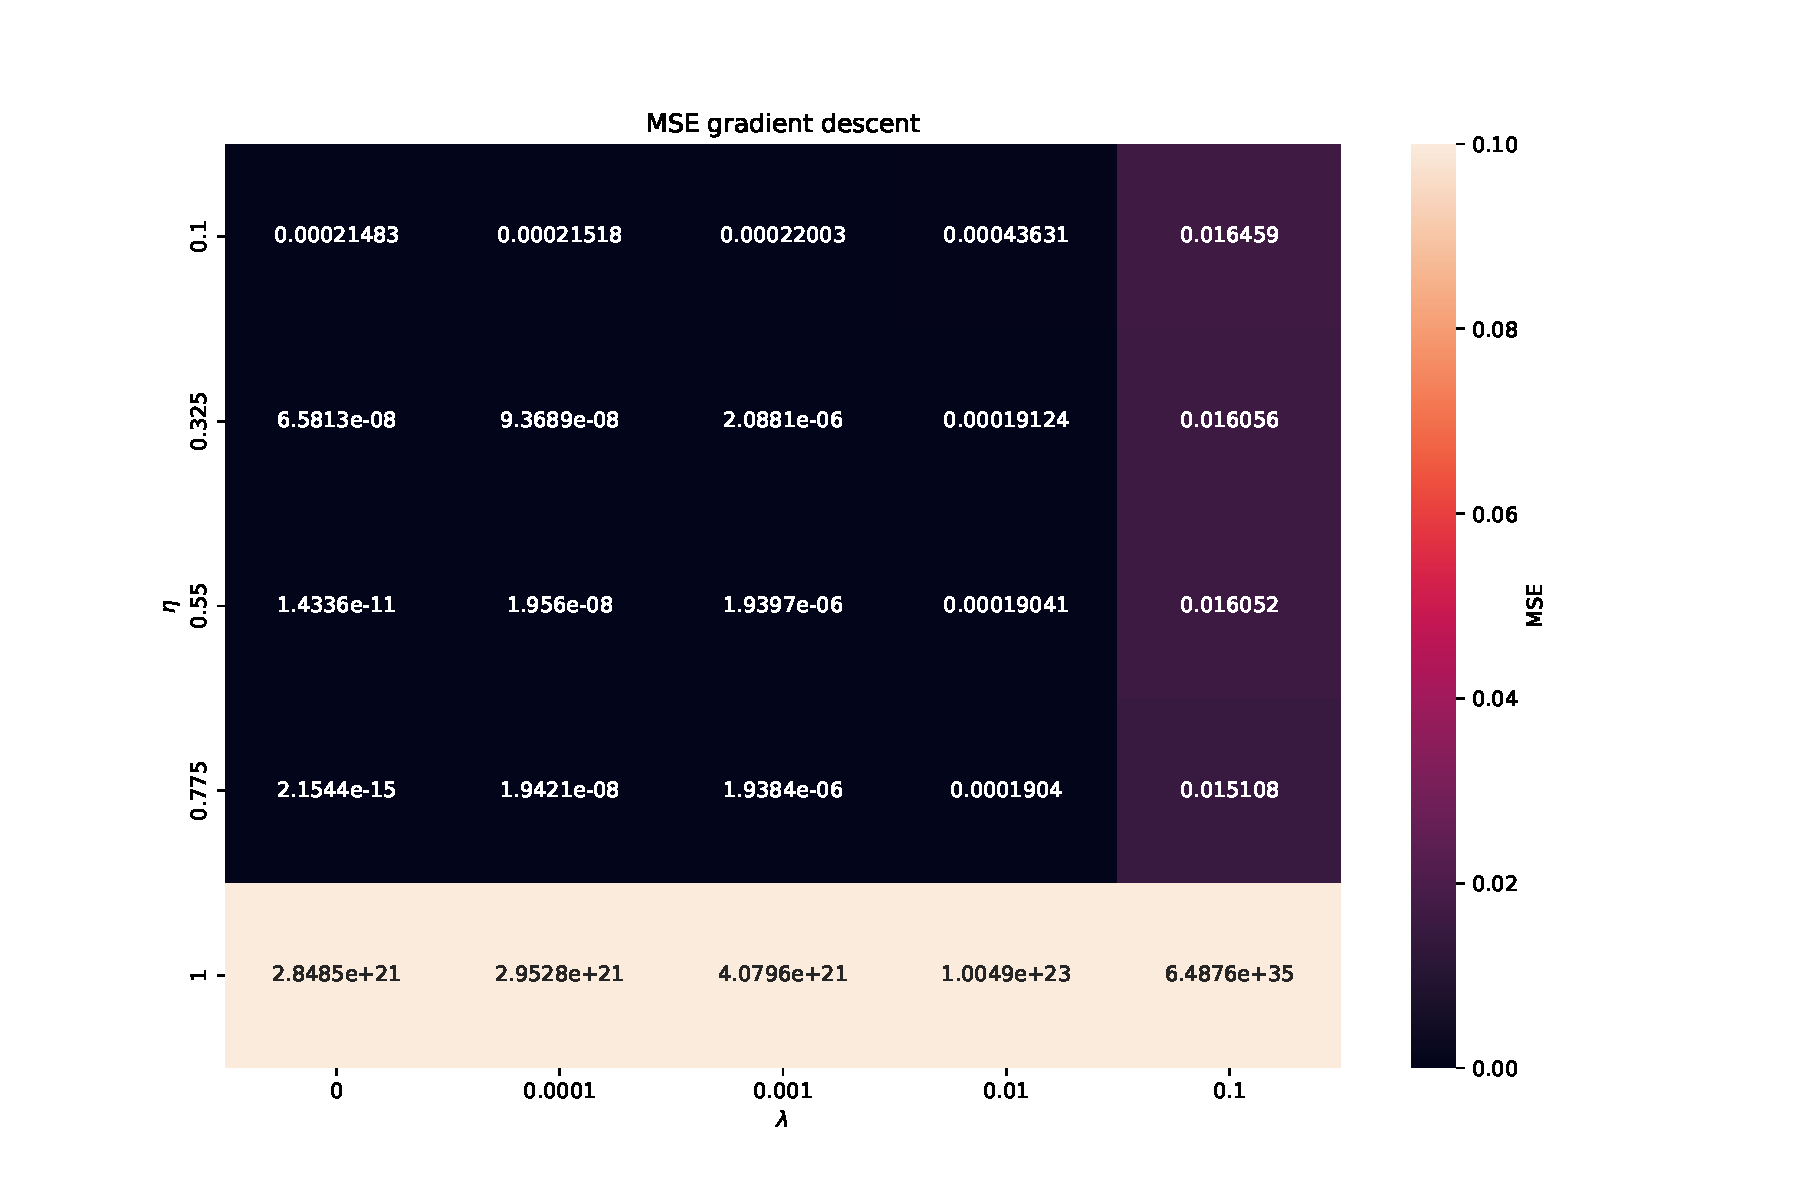
\includegraphics[width=0.8\textwidth]{Figures/PartA/gd_MSE(eta,lmb)}
\caption{Plain gradient descent MSE as a function of \(\eta \) and \(\lambda \).}
\label{fig:gd_MSE-eta-lmb-}
\end{figure}

\begin{figure}[H]
\centering
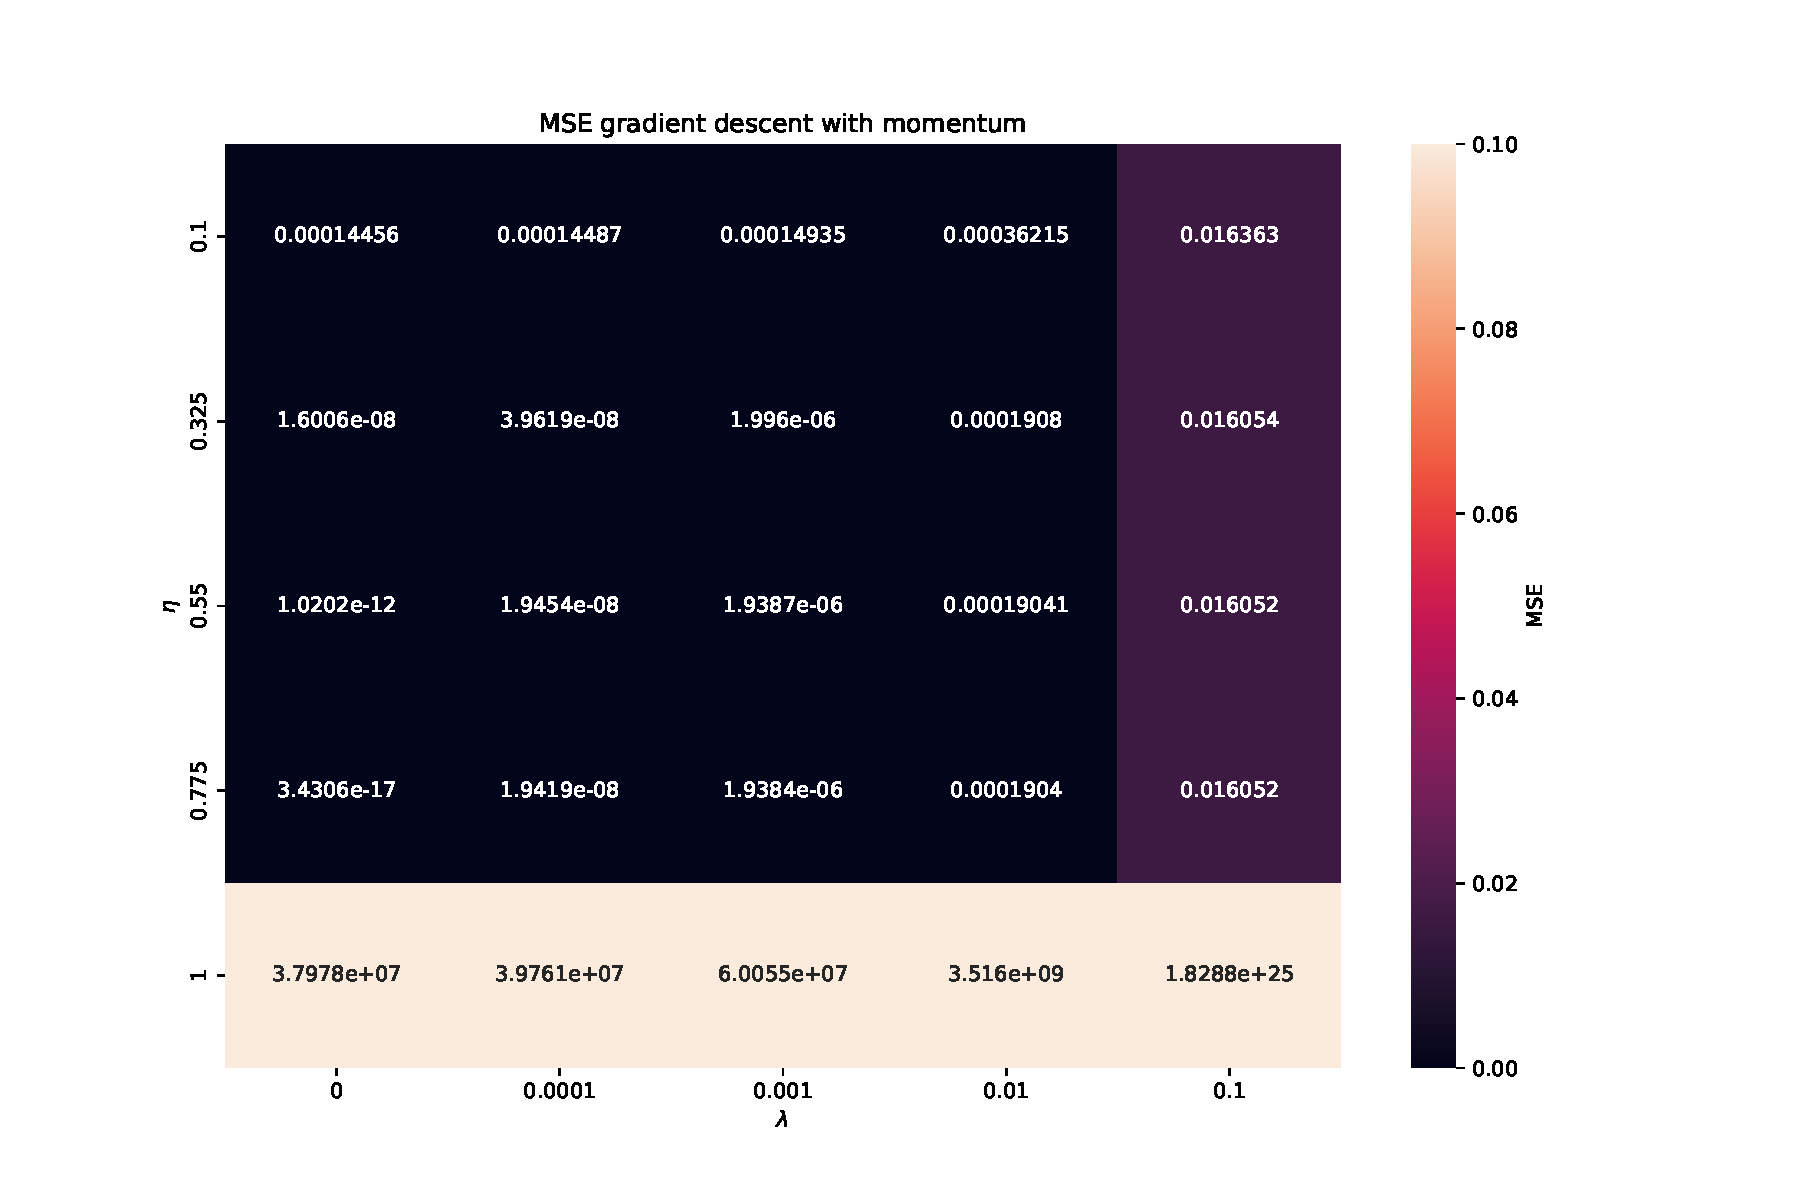
\includegraphics[width=0.8\textwidth]{Figures/PartA/gdm_MSE(eta,lmb)}
\caption{Gradient descent with momentum MSE as a function of \(\eta \) and \(\lambda \).}
\label{fig:gdm_MSE-eta-lmb-}
\end{figure}

\begin{figure}[H]
\centering
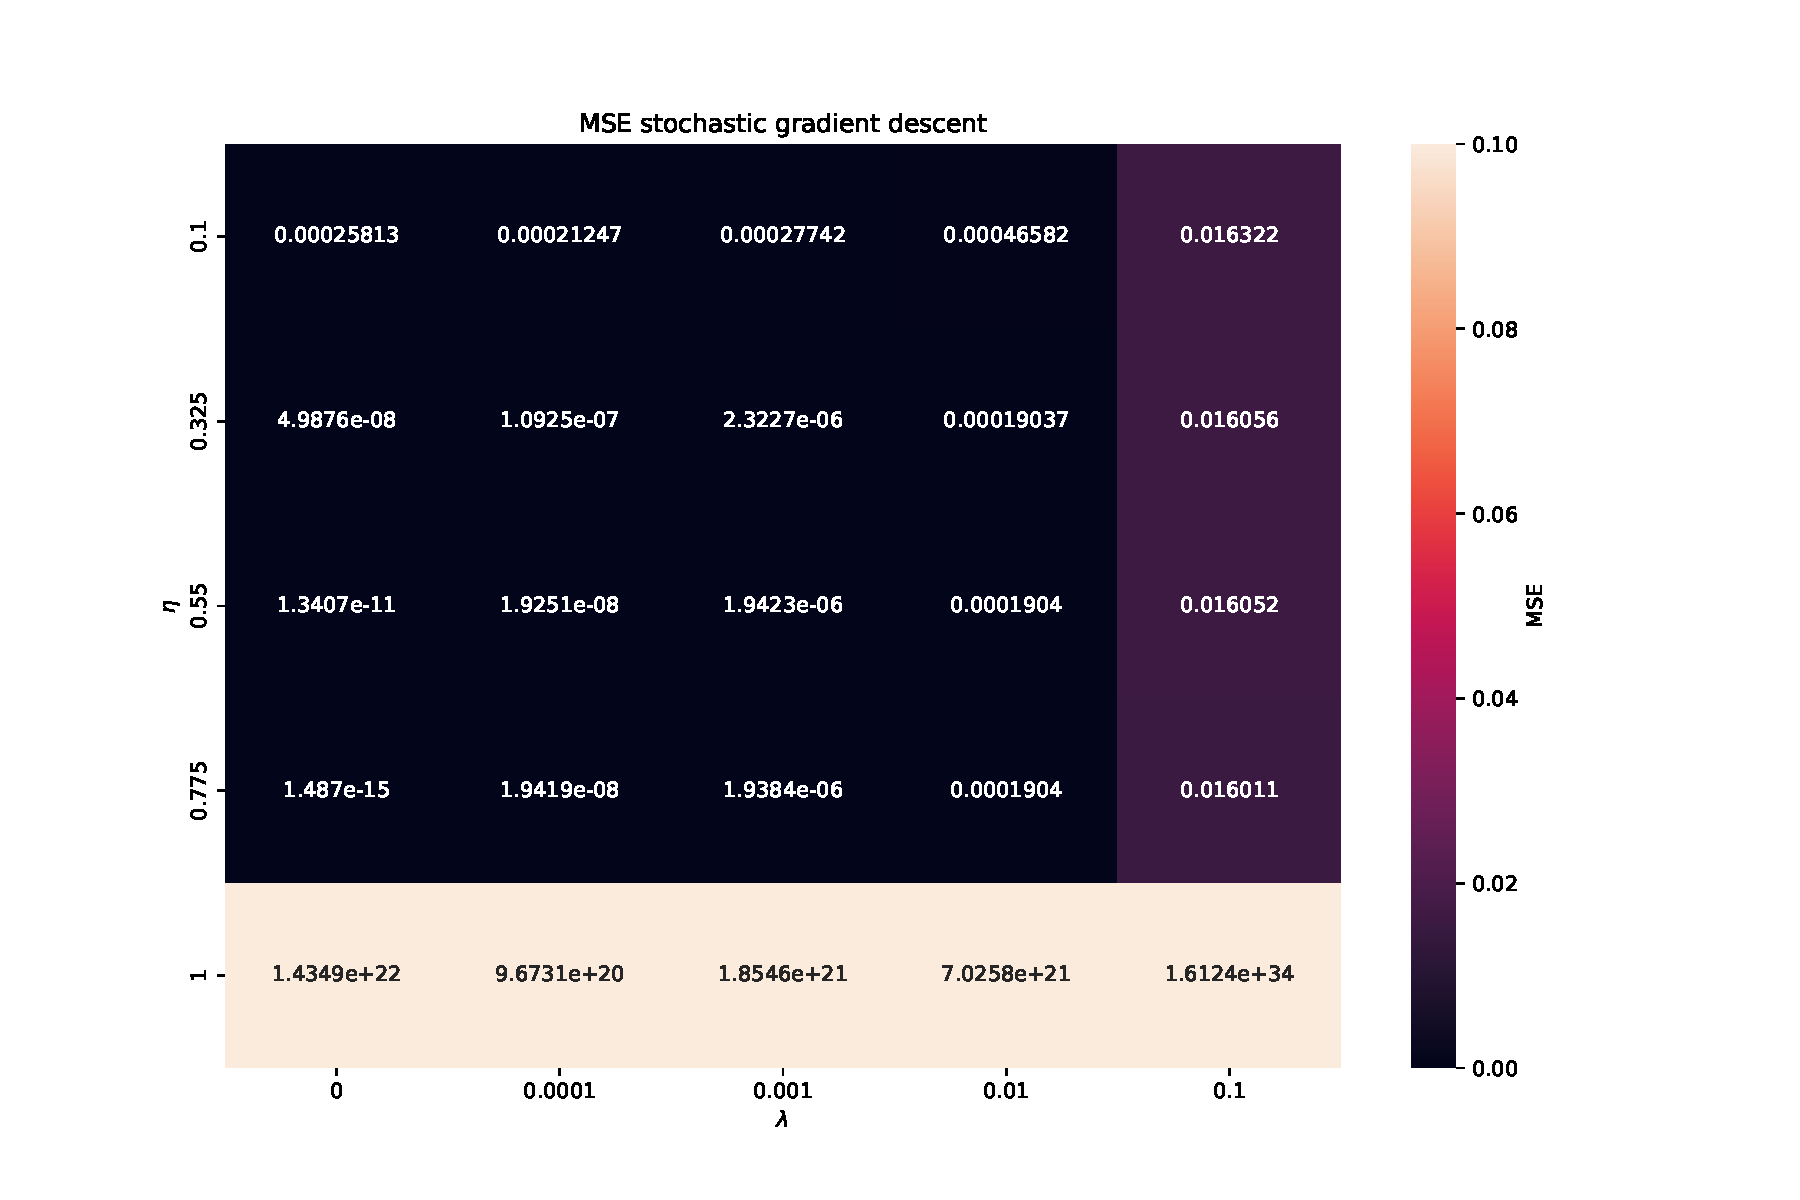
\includegraphics[width=0.8\textwidth]{Figures/PartA/sgd_MSE(eta,lmb)}
\caption{Plain stochastic gradient descent MSE as a function of \(\eta \) and \(\lambda \).}
\label{fig:sgd_MSE-eta-lmb-}
\end{figure}

\begin{figure}[H]
\centering
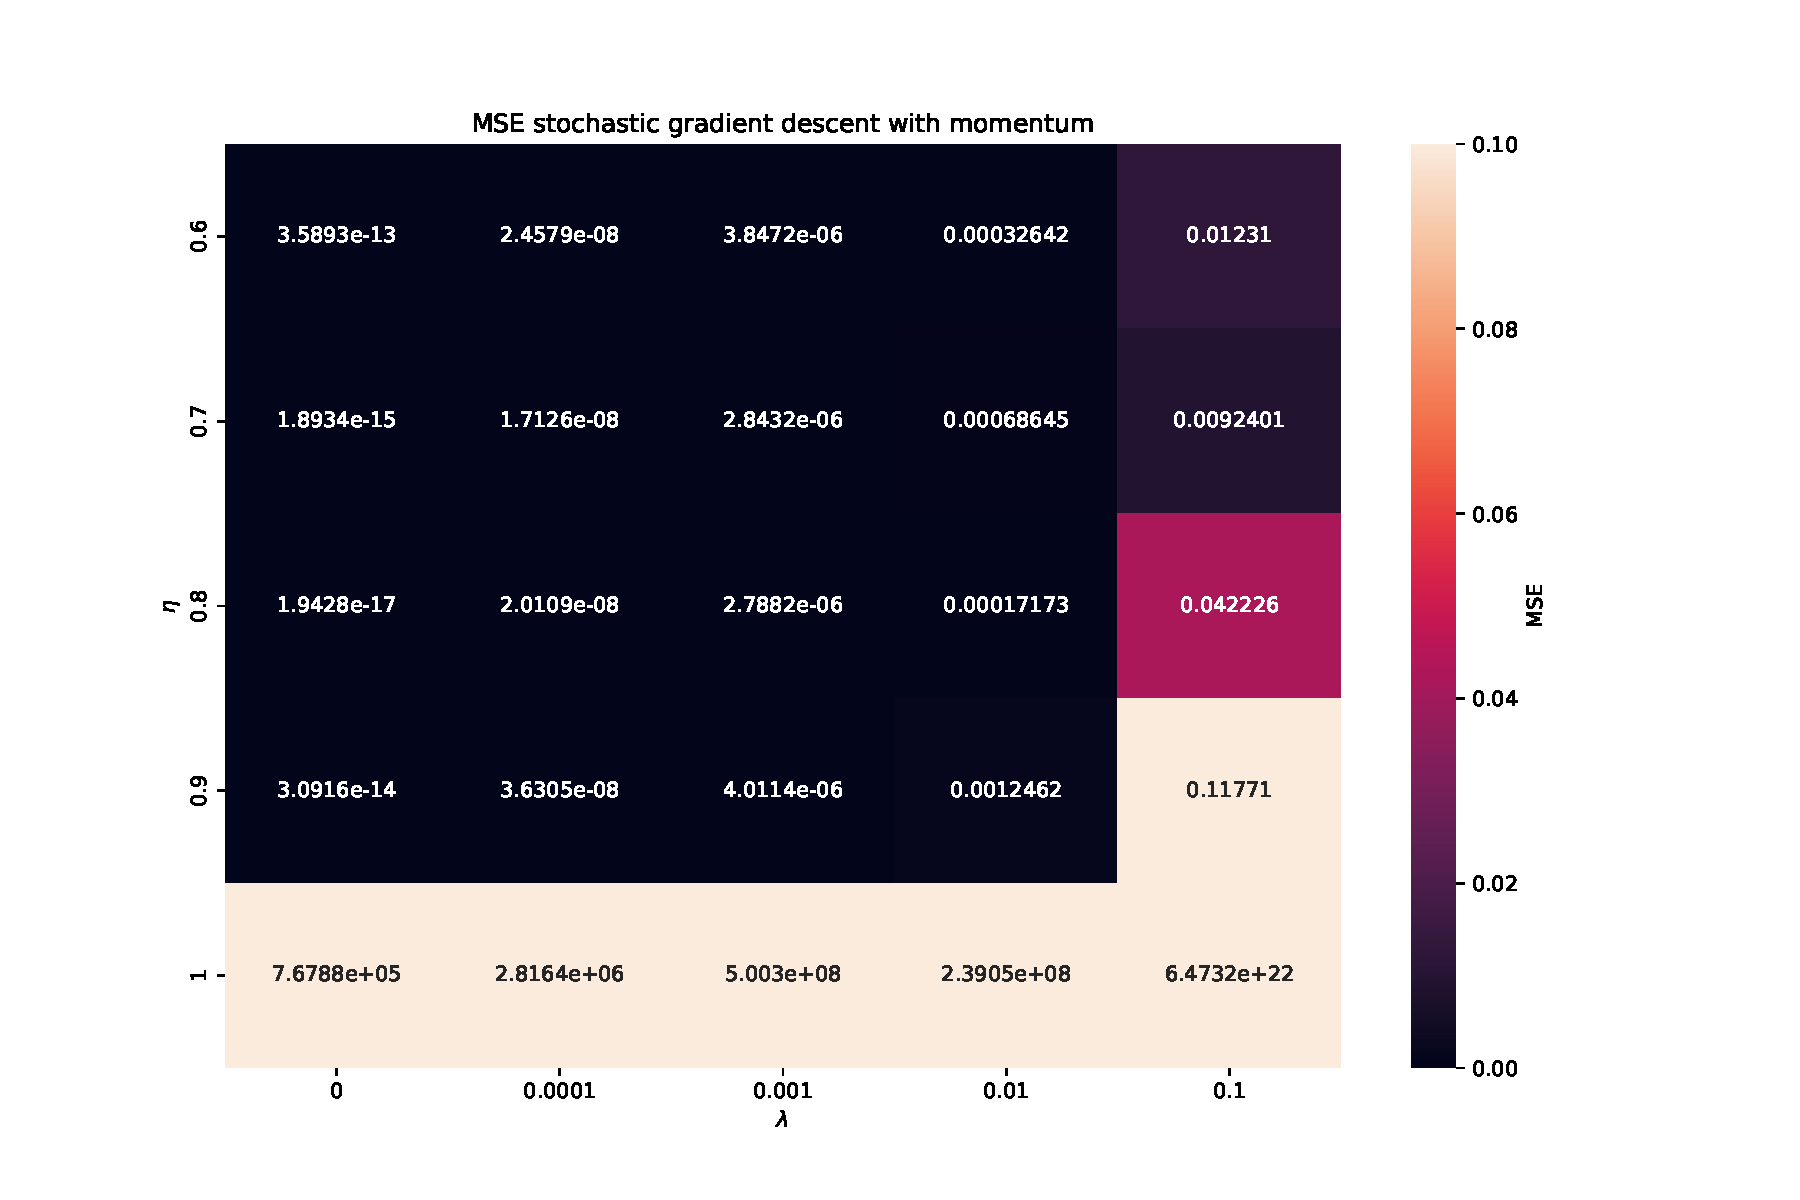
\includegraphics[width=0.8\textwidth]{Figures/PartA/sgdm_MSE(eta,lmb)}
\caption{Stochastic gradient descent with momentum MSE as a function of \(\eta \) and \(\lambda \).}
\label{fig:sgdm_MSE-eta-lmb-}
\end{figure}

Figure \ref{fig:gd_MSE-eta-lmb-}-\ref{fig:sgdm_MSE-eta-lmb-} shows MSE scores for 
stochastic gradient descent without ans with momentum, and stochastic gradient descent
without and with momentum, respectively. 
different learning rates \(\eta \) and L2-regularzation parameters \(\lambda \). 


\begin{figure}[H]
\centering
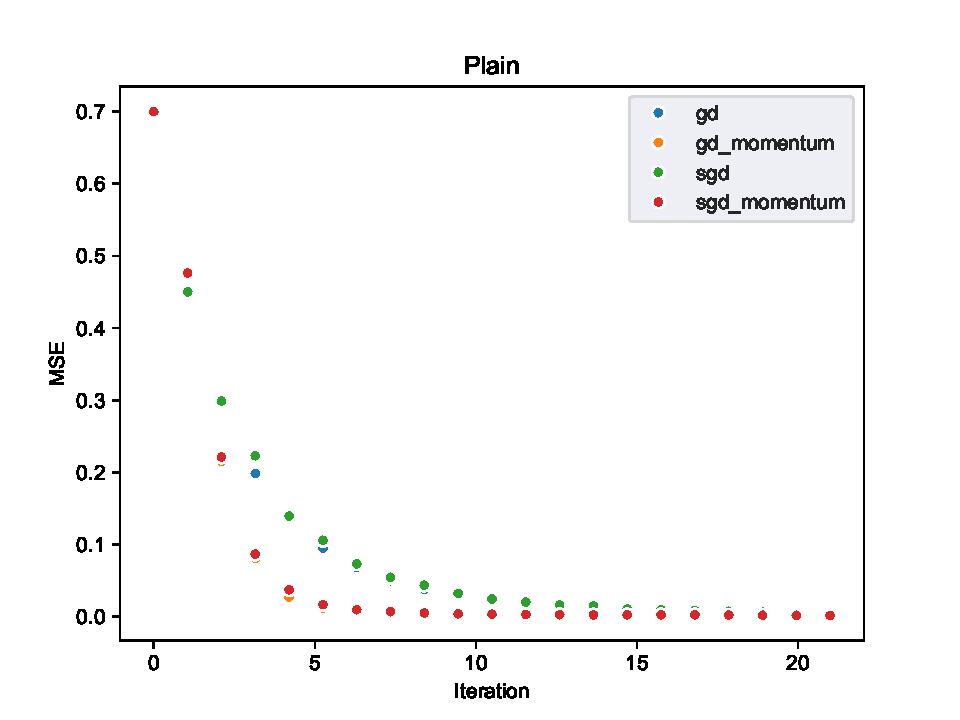
\includegraphics[width=0.8\textwidth]{Figures/PartA/PlainMSE(iter).pdf}
\caption{MSE as a function of iterations for plain and stochastic gradient descent with and without momentum}
\label{fig:PlainMSE-iter-pdf}
\end{figure}

\begin{figure}[H]
\centering
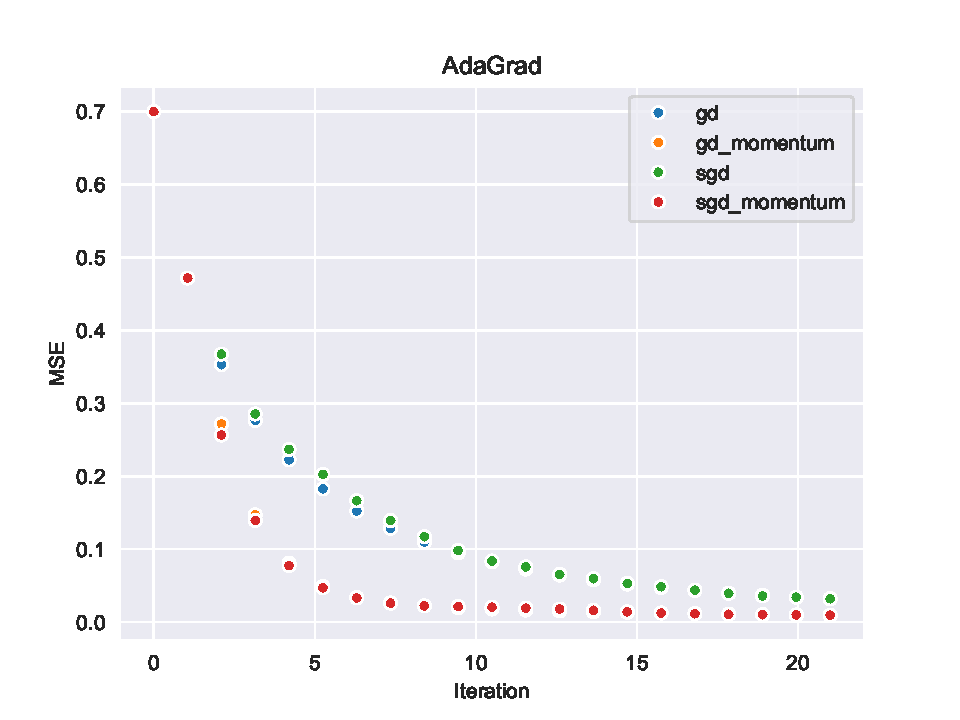
\includegraphics[width=0.8\textwidth]{Figures/PartA/AdaGradMSE(iter).pdf}
\caption{MSE as a function of iterations using tuning method AdaGrad for plain and stochastic gradient descent with and without momentum}
\label{fig:AdaGradMSE-iter-pdf}
\end{figure}

\begin{figure}[H]
\centering
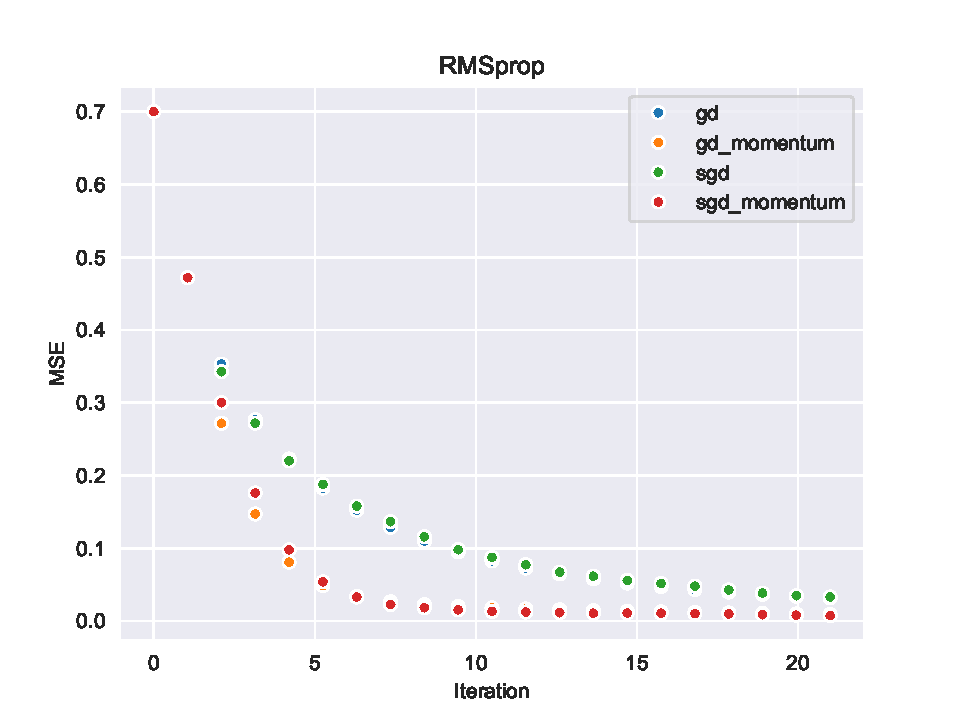
\includegraphics[width=0.8\textwidth]{Figures/PartA/RMSpropMSE(iter).pdf}
\caption{MSE as a function of iterations using tuning method RMSprop for plain and stochastic gradient descent with and without momentum}
\label{fig:RMSpropMSE-iter-pdf}
\end{figure}

\begin{figure}[H]
\centering
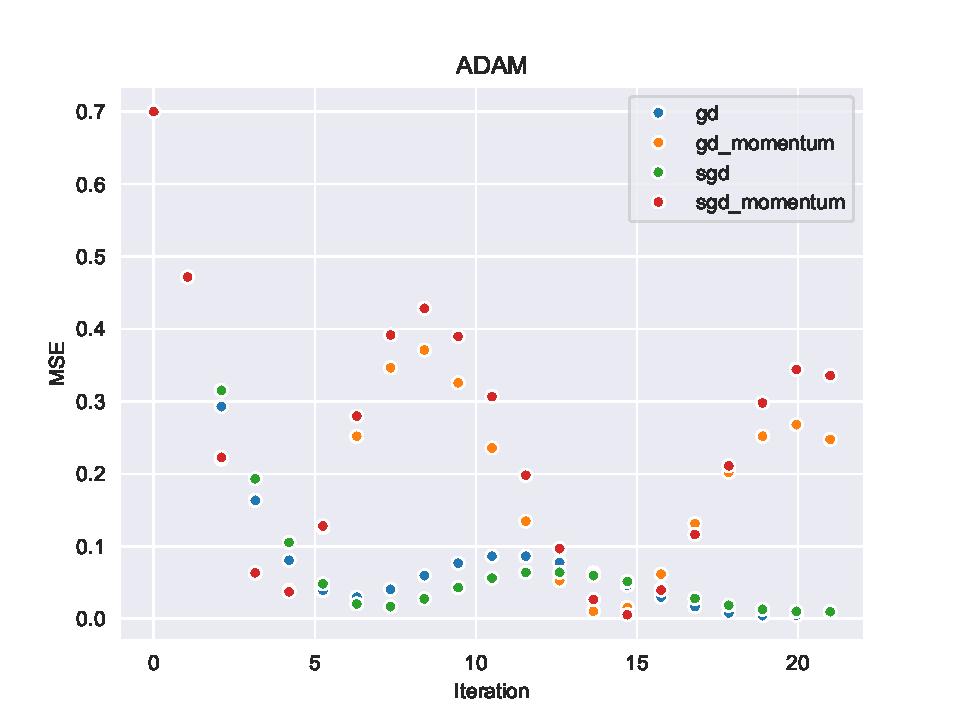
\includegraphics[width=0.8\textwidth]{Figures/PartA/ADAMMSE(iter).pdf}
\caption{MSE as a function of iterations using tuning method ADAM for plain and stochastic gradient descent with and without momentum}
\label{fig:ADAMMSE-iter-pdf}
\end{figure}



\begin{figure}[H]
\centering
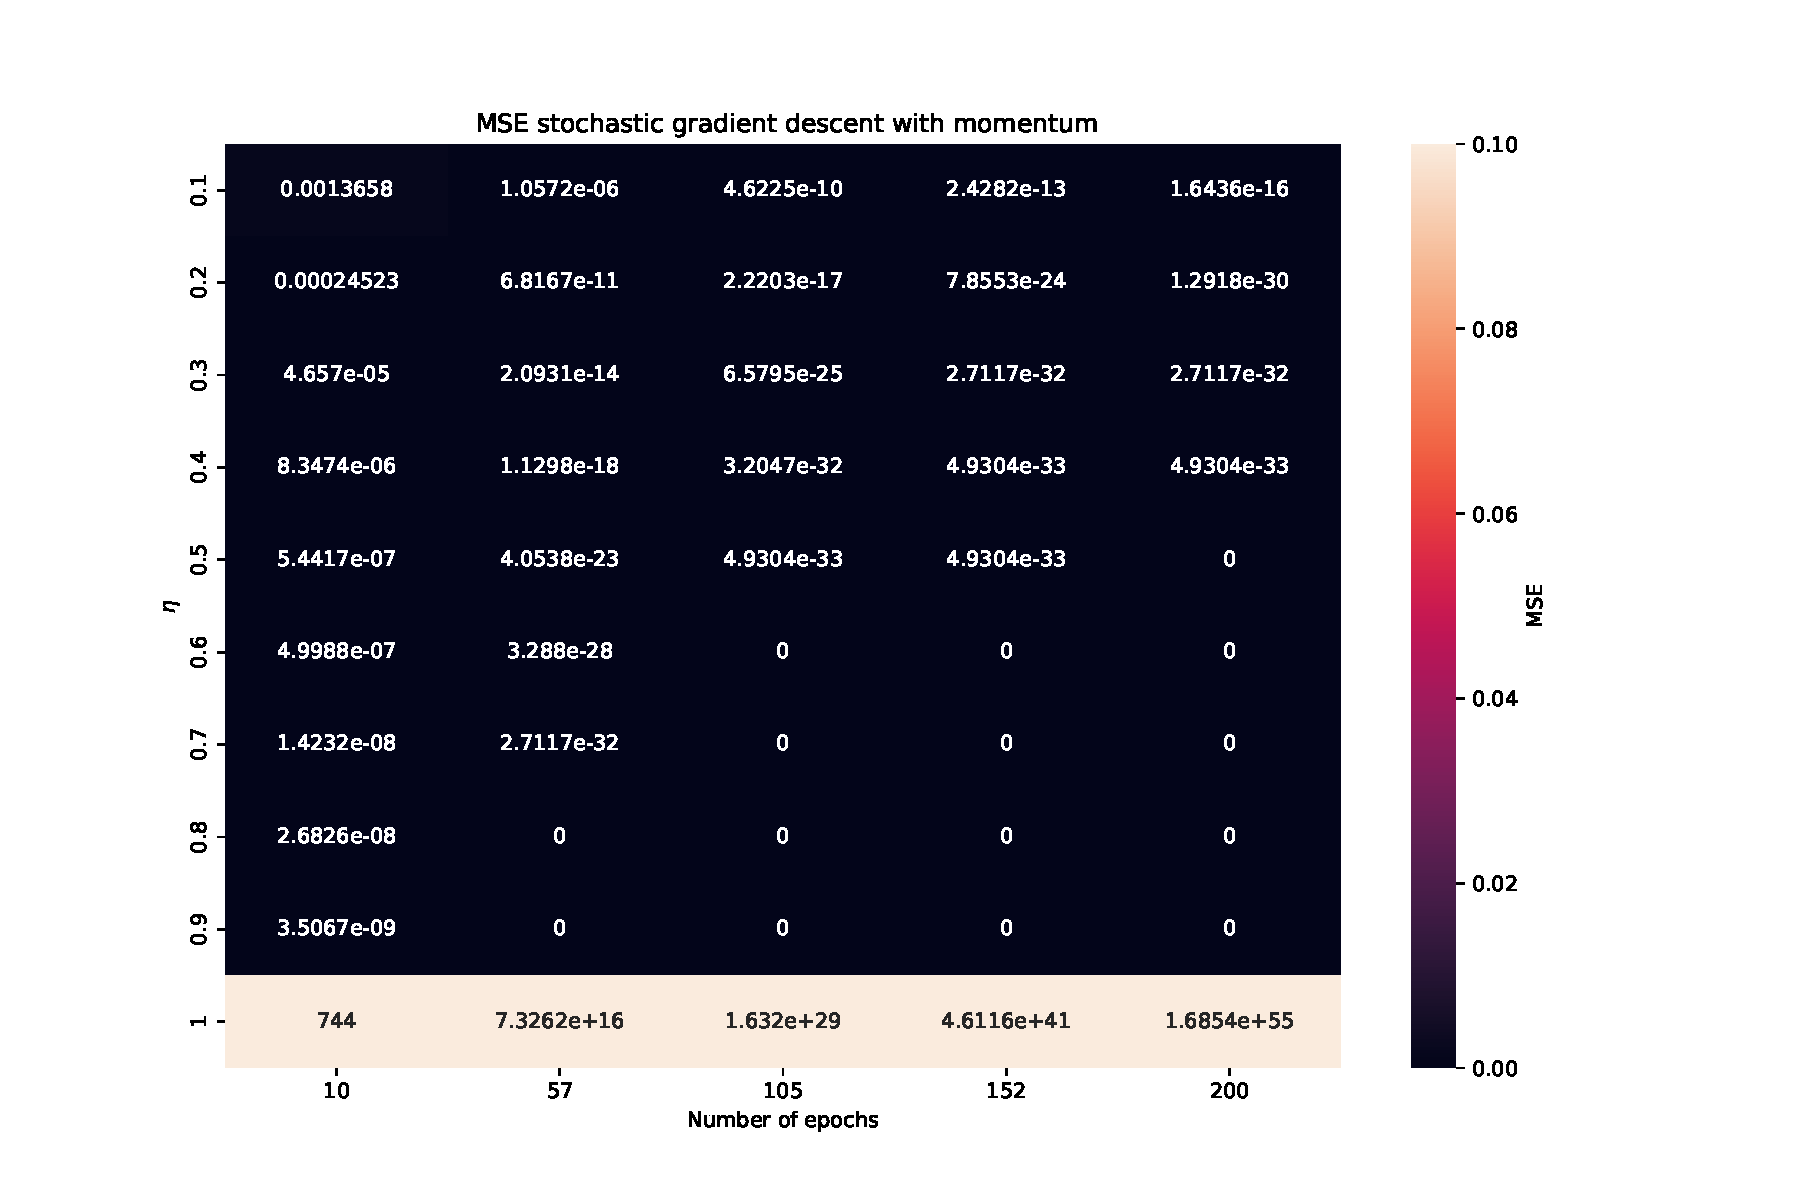
\includegraphics[width=0.8\textwidth]{Figures/PartA/_sgdm_MSE(eta,epochs)}
\caption{Stochastic gradient descent with momentum MSE as a function of epoch number and \(\eta \)	 }
\label{fig:_sgdm_MSE-eta-epochs-}
\end{figure}

\begin{figure}[H]
\centering
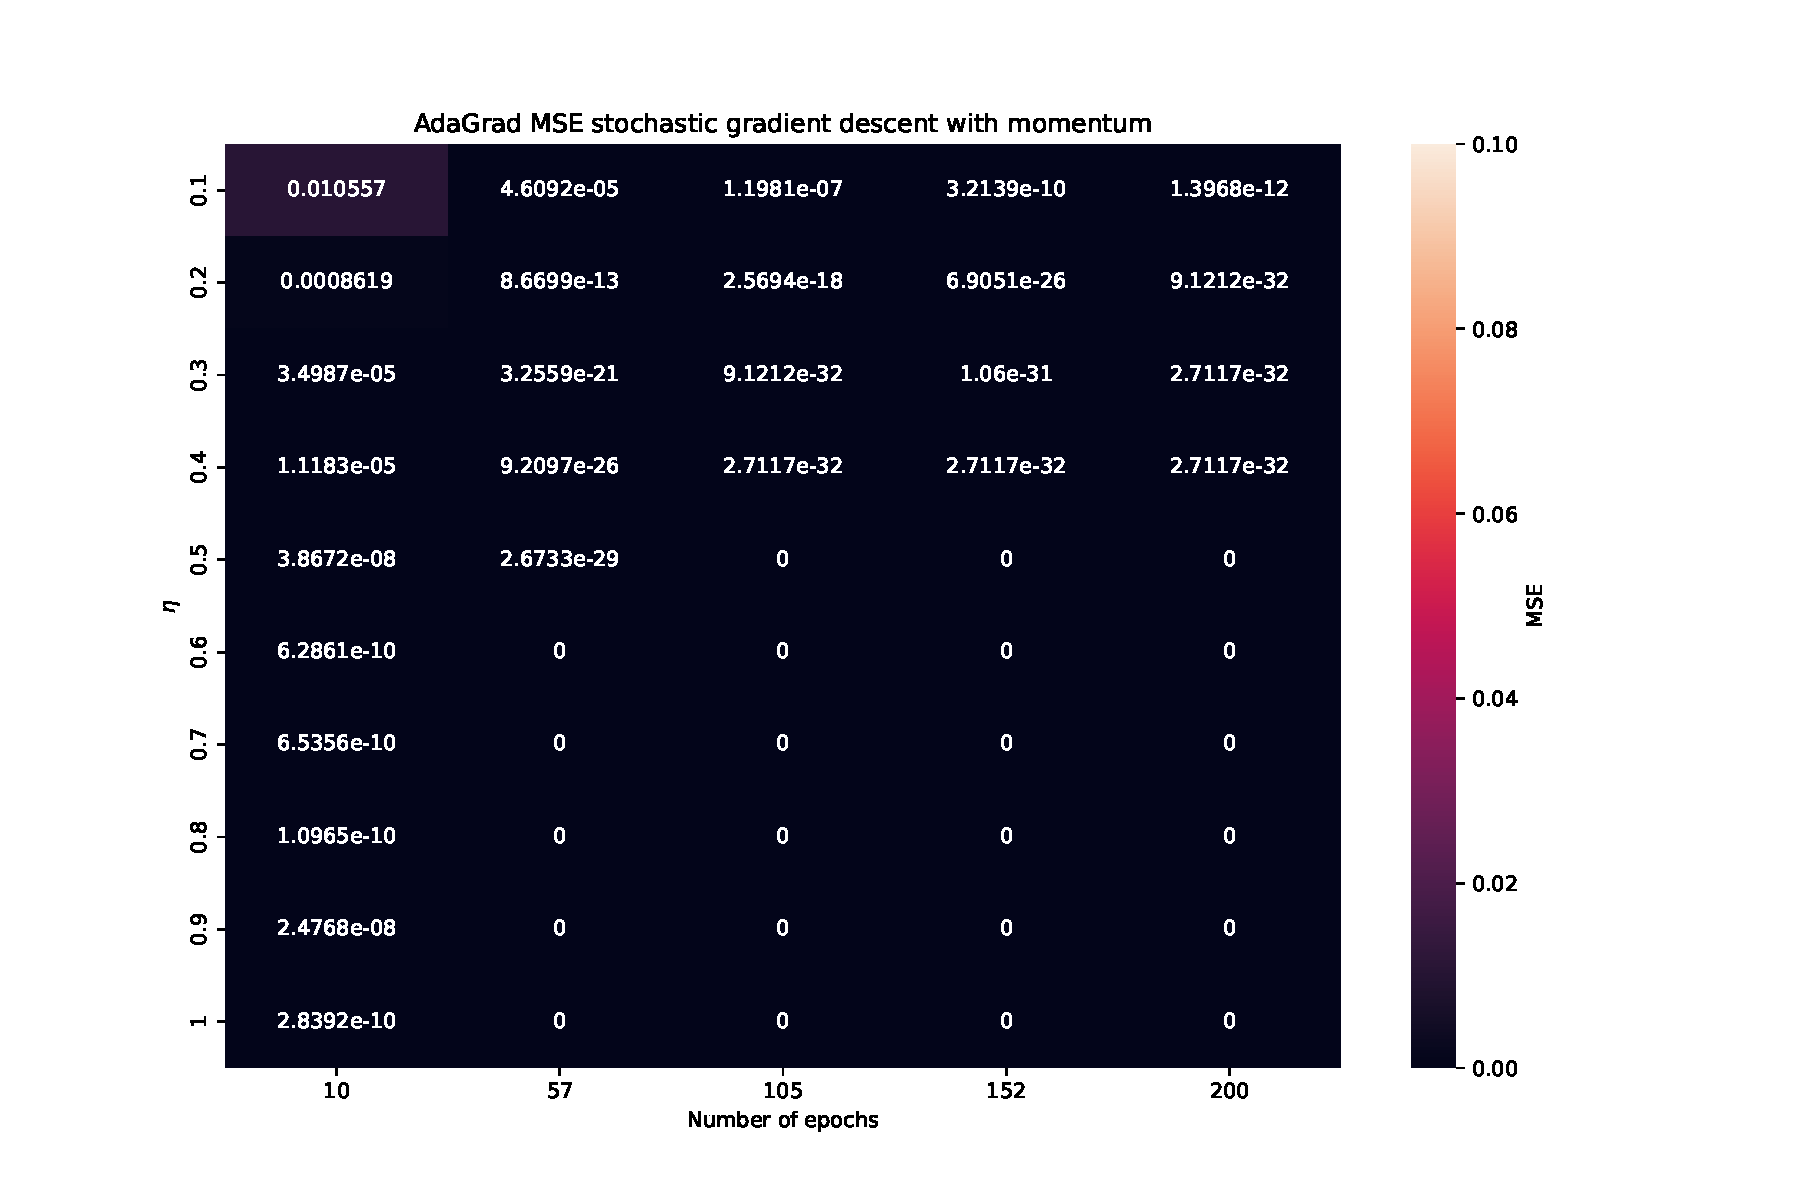
\includegraphics[width=0.8\textwidth]{Figures/PartA/AdaGrad_sgdm_MSE(eta,epochs)}
\caption{Stochastic gradient descent, with momentum and tuning method AdaGrad, MSE as a function of epoch number and \(\eta \)	 }
\label{fig:AdaGrad_sgdm_MSE-eta-epochs-}
\end{figure}

\begin{figure}[H]
\centering
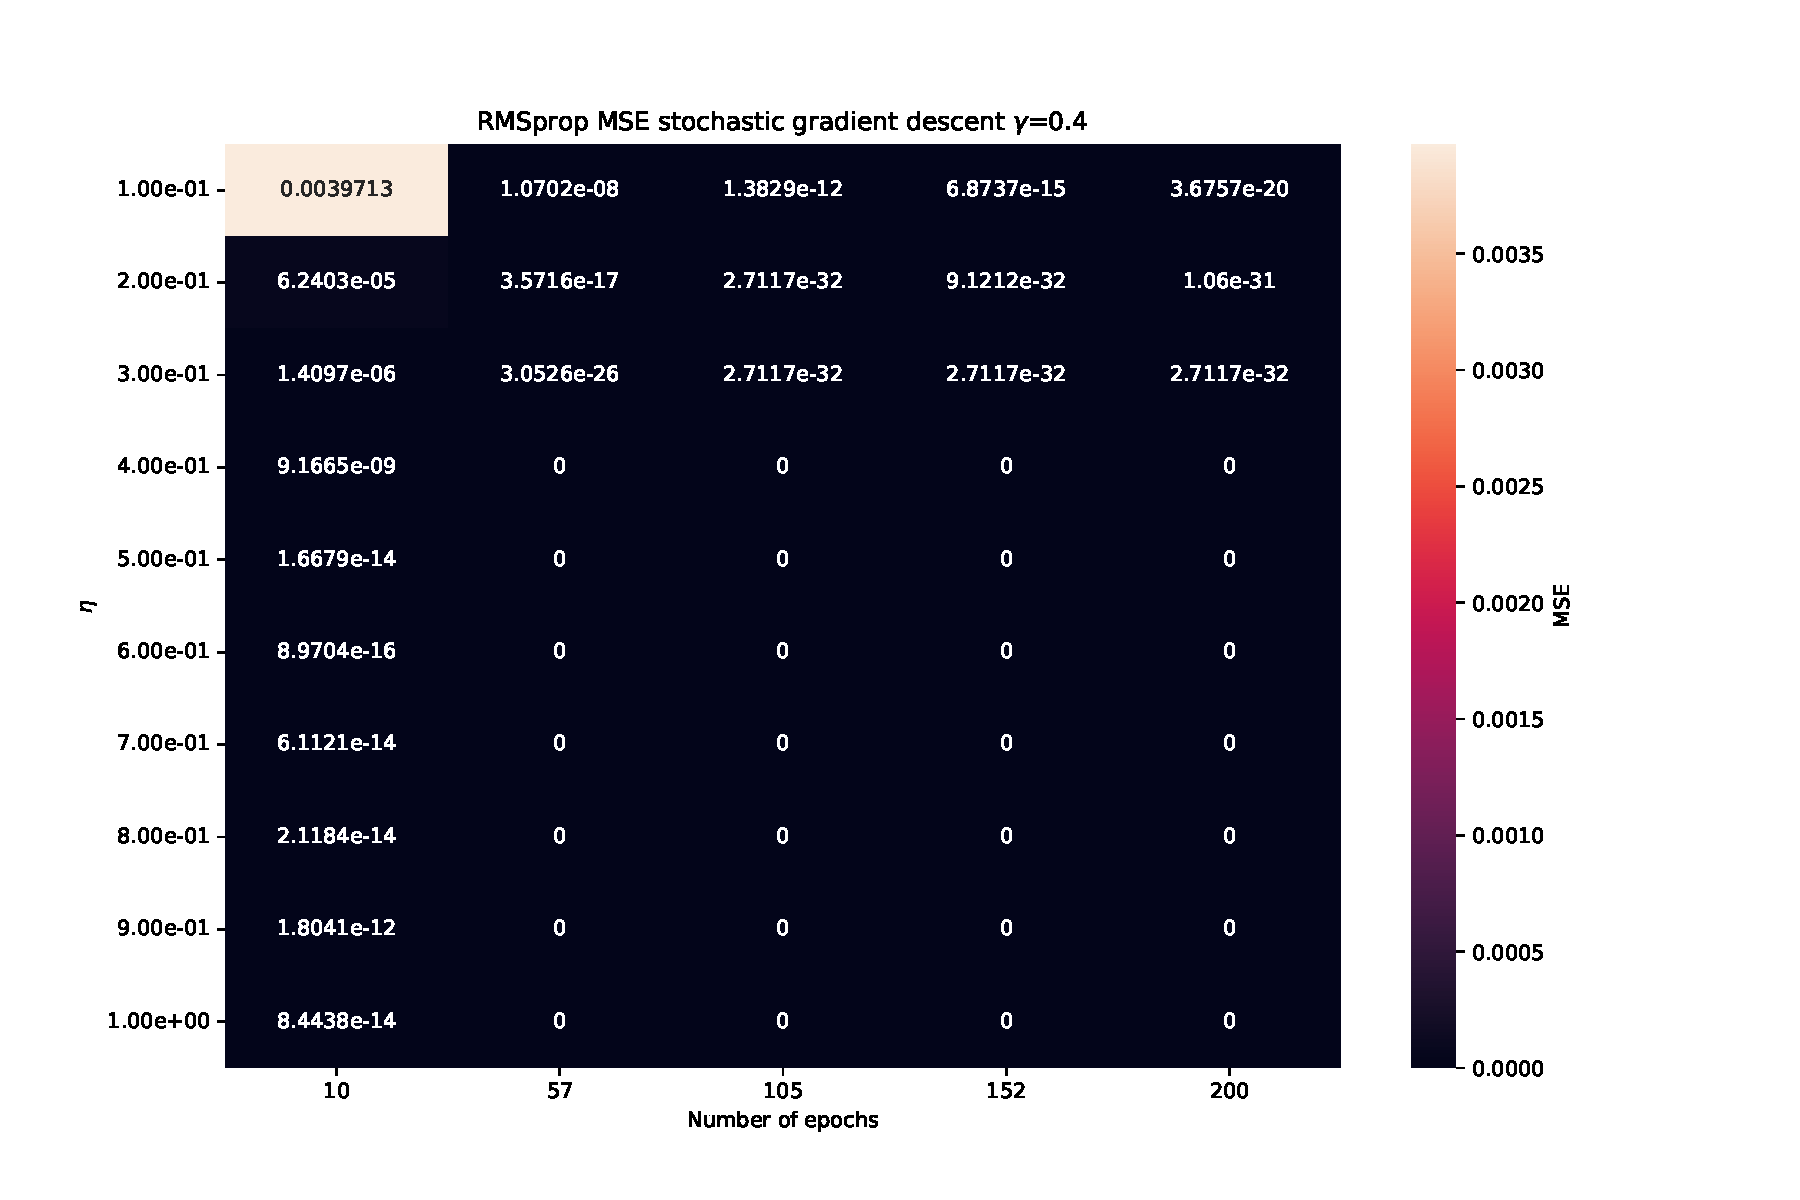
\includegraphics[width=0.8\textwidth]{Figures/PartA/RMSprop_sgdm_MSE(eta,epochs)}
\caption{Stochastic gradient descent, with momentum and tuning method RMS\_prop, MSE as a function of epoch number and \(\eta \)	 }
\label{fig:RMSprop_sgdm_MSE-eta-epochs-}
\end{figure}

\begin{figure}[H]
\centering
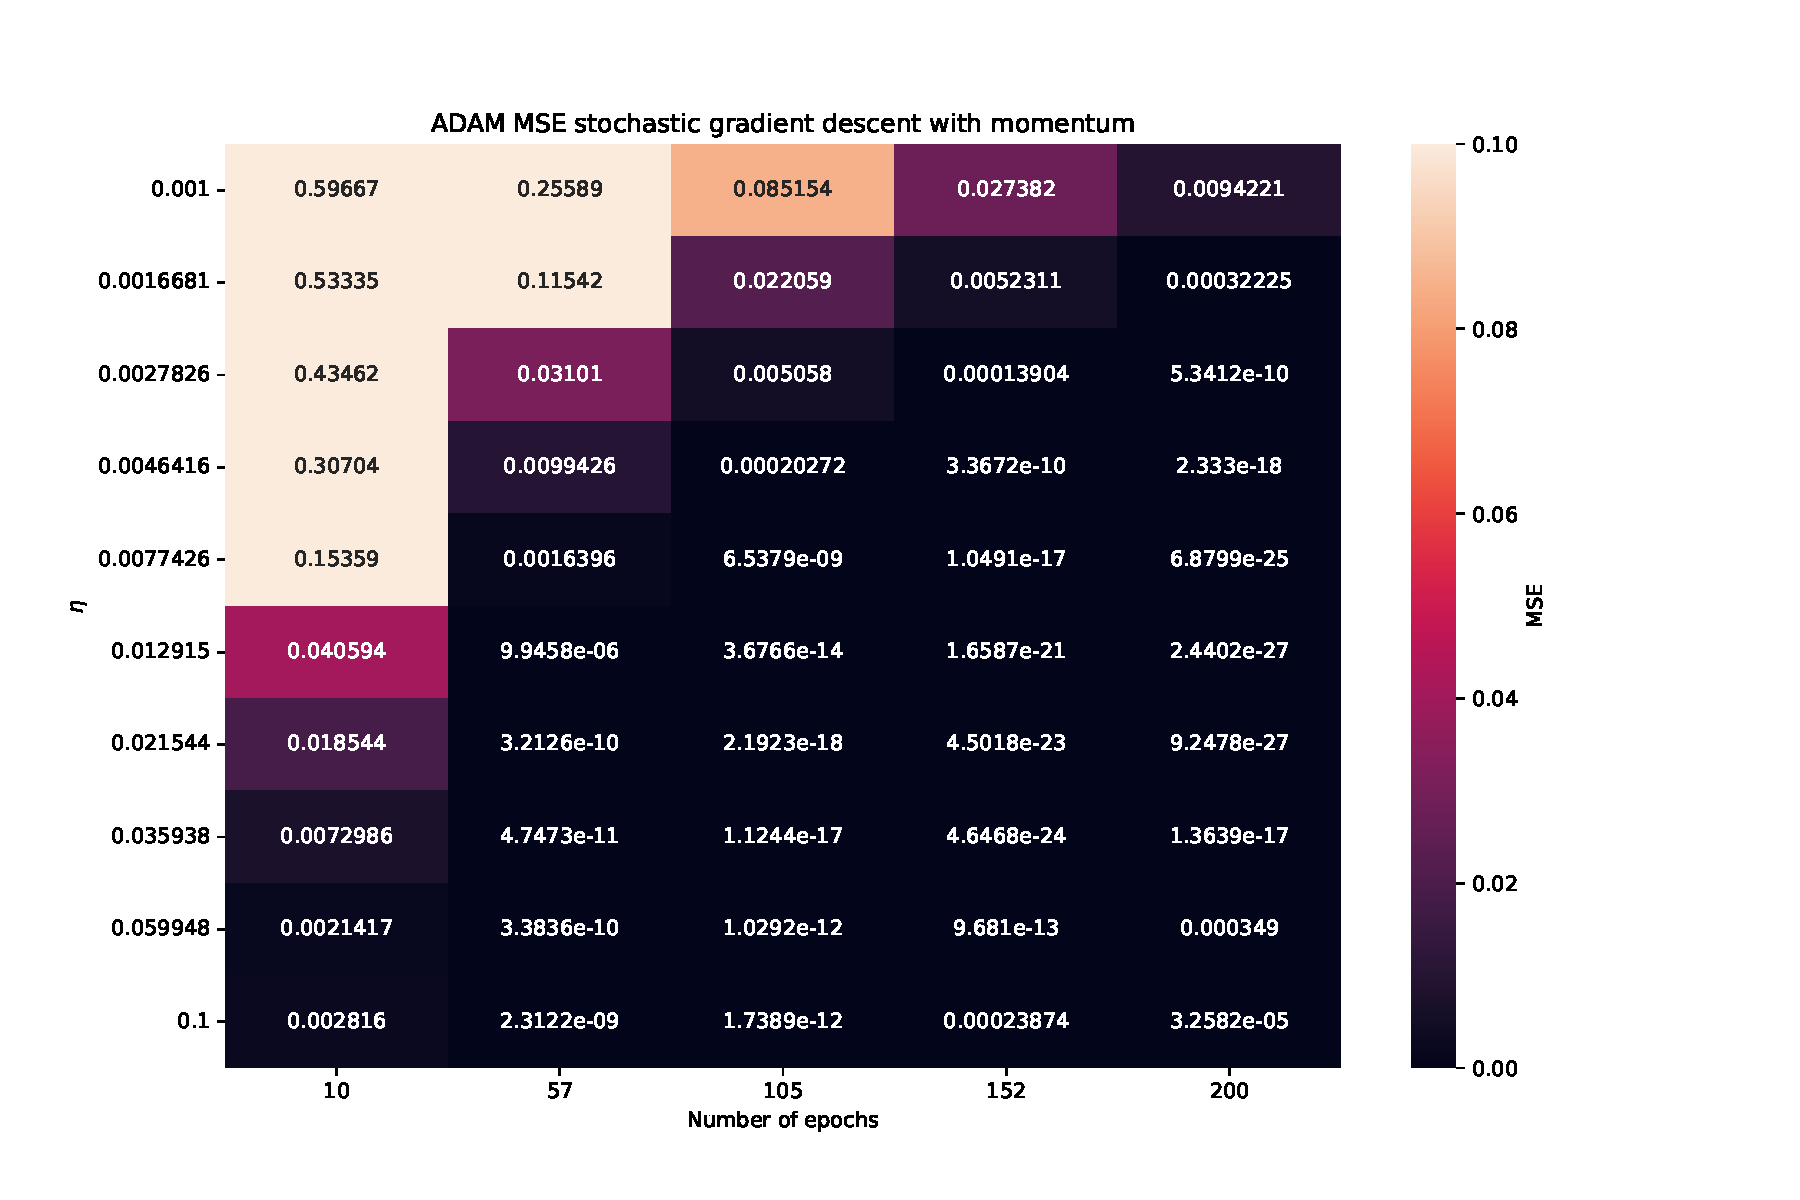
\includegraphics[width=0.8\textwidth]{Figures/PartA/ADAM_sgdm_MSE(eta,epochs)}
\caption{Stochastic gradient descent, with momentum and tuning method ADAM, MSE as a function of epoch number and \(\eta \)	 }
\label{fig:ADAM_sgdm_MSE-eta-epochs-}
\end{figure}


\subsection{Neural Network Regression}

\begin{figure}[htpb]
\begin{subfigure}{.5\textwidth}
  \centering
  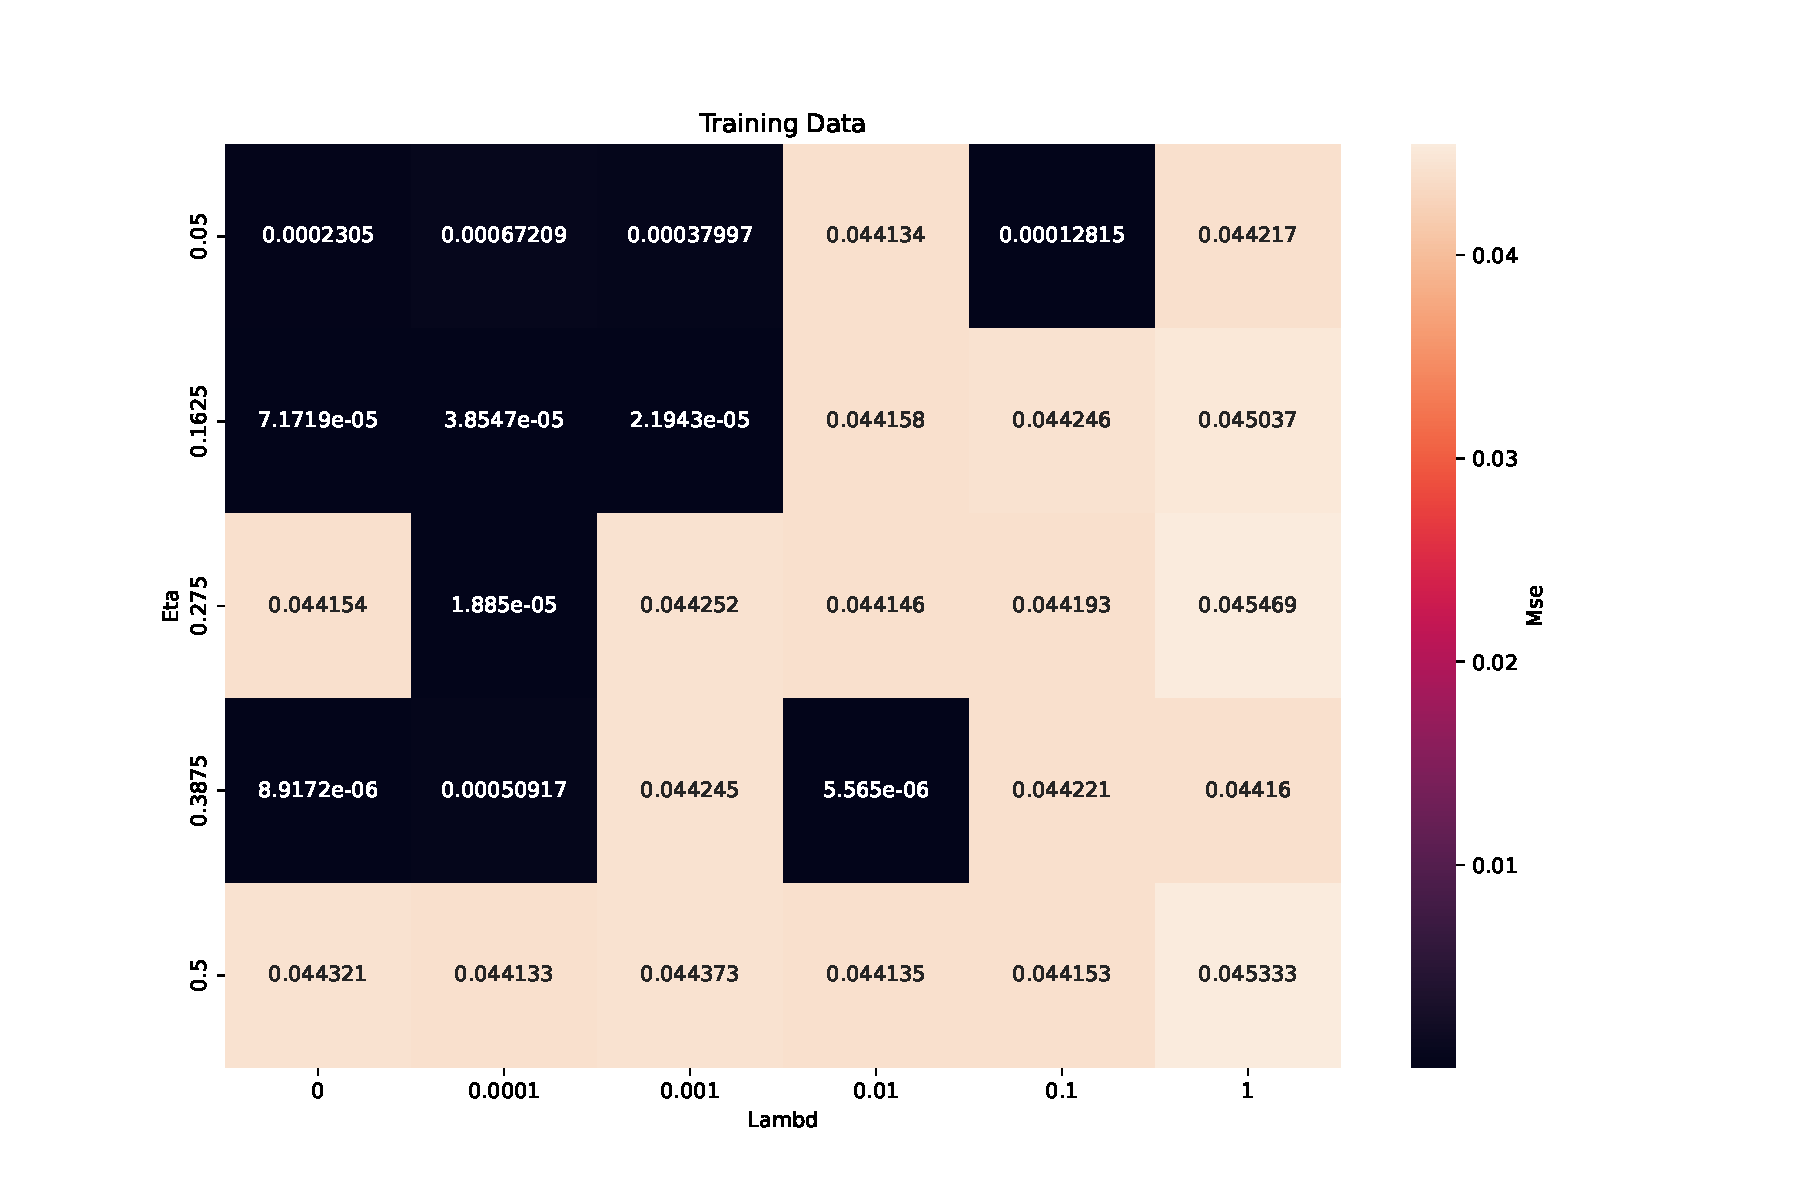
\includegraphics[width=1.2\linewidth]{Figures/PartB/train_sigmoid_MSE(eta,lmb)}
  \caption{Train MSE}
  \label{fig:train_sigmoid_MSE-eta-lmb-}
\end{subfigure}%
\begin{subfigure}{.5\textwidth}
  \centering
  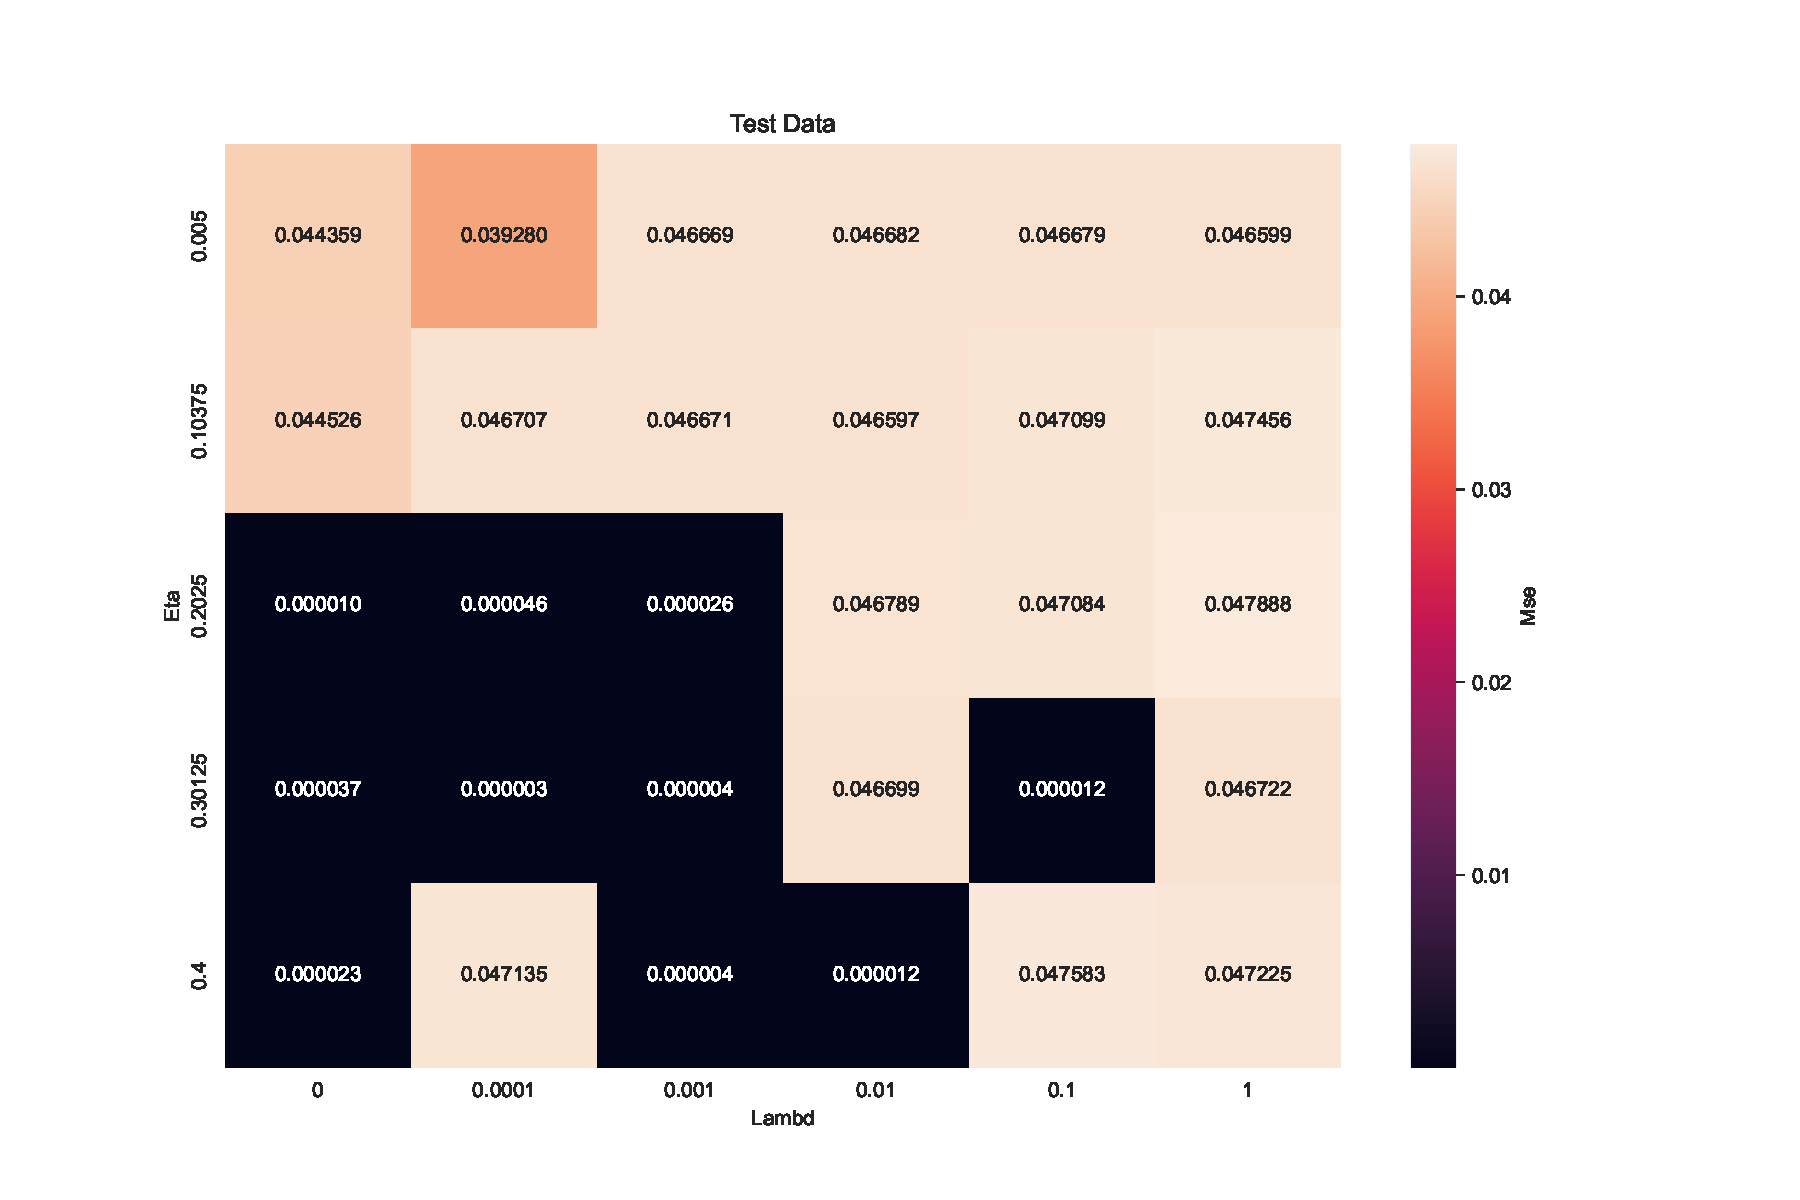
\includegraphics[width=1.2\linewidth]{Figures/PartB/test_sigmoid_MSE(eta,lmb)}
  \caption{Test MSE}
  \label{fig:test_sigmoid_MSE-eta-lmb-}
\end{subfigure}
\caption{Neural network with activation function Sigmoid MSE as a function of \(\eta \) and \(\lambda \) }
\label{fig:Sigmoid_MSE}
\end{figure}

\begin{figure}[htpb]
\begin{subfigure}{.5\textwidth}
  \centering
  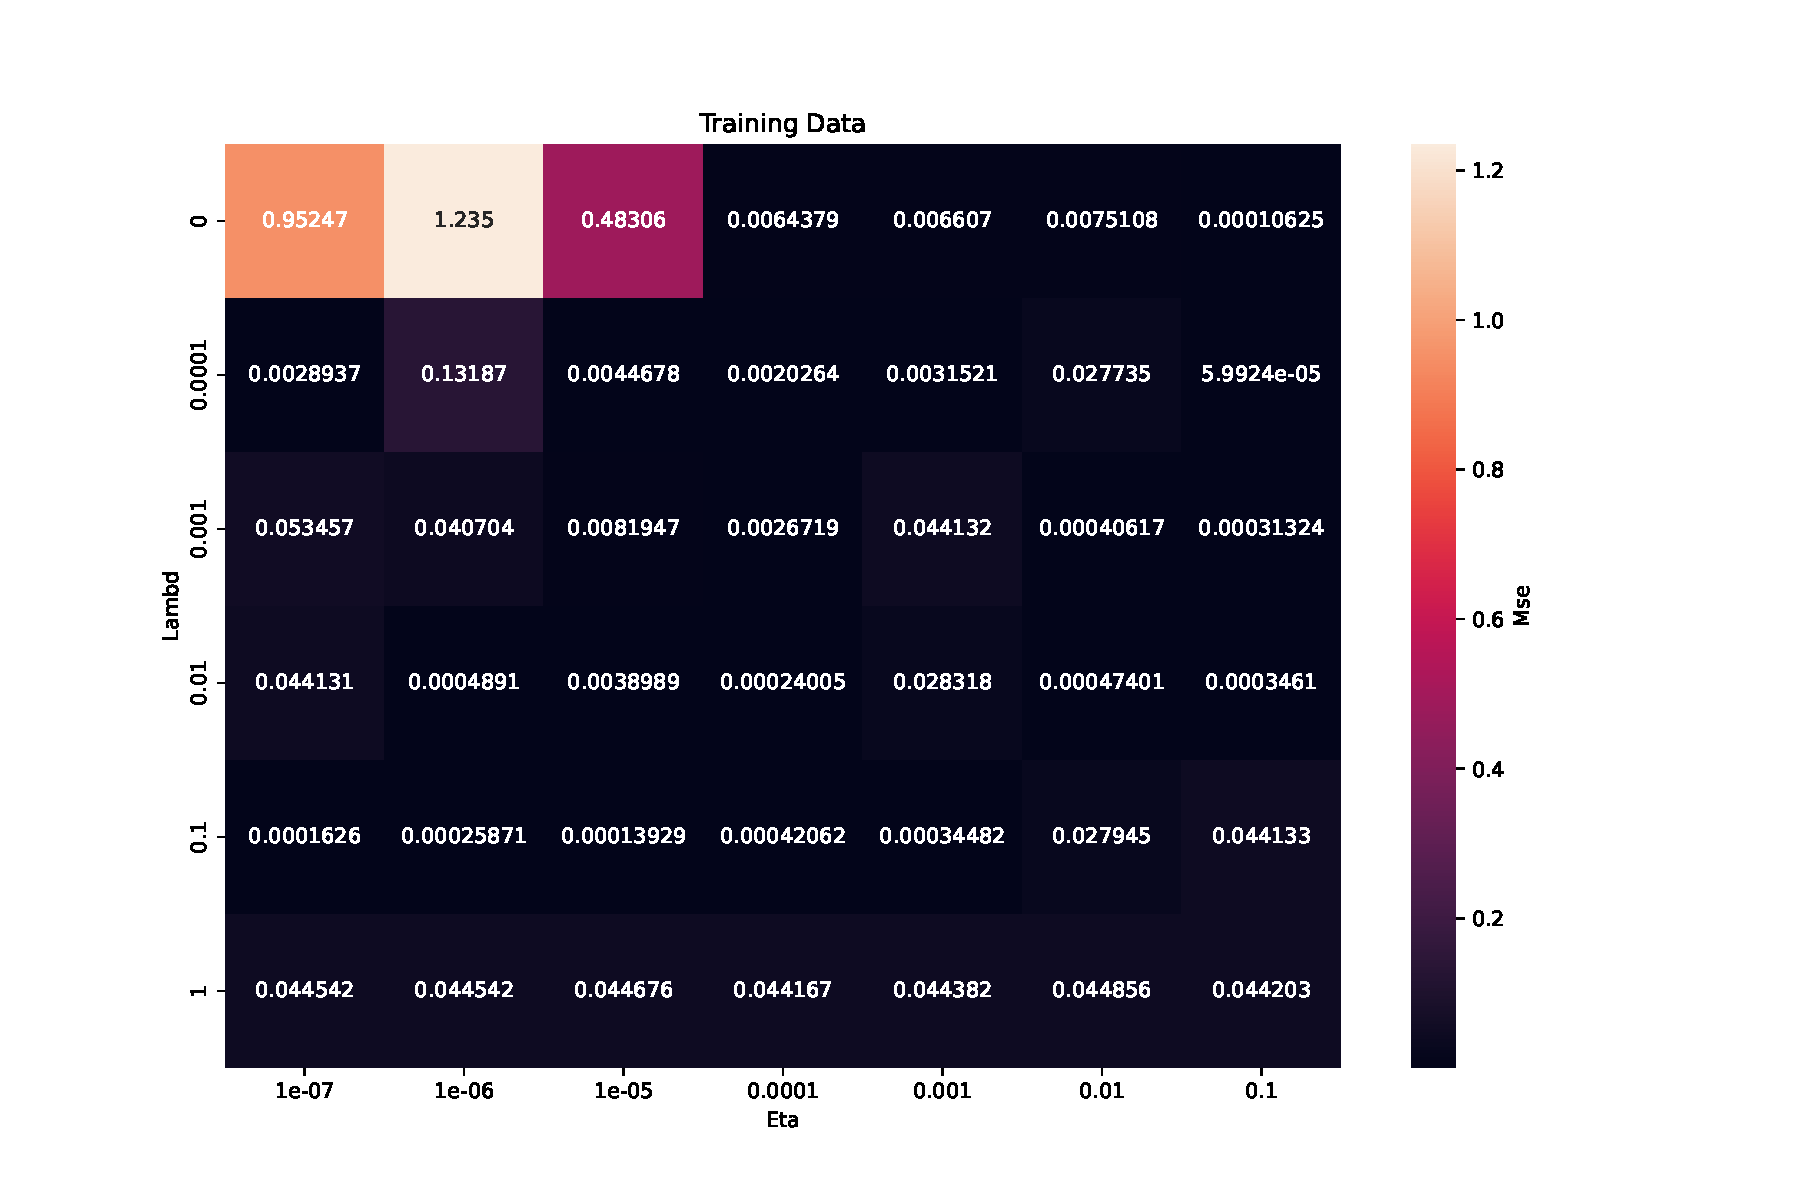
\includegraphics[width=1.2\linewidth]{Figures/PartB/train_relu_MSE(eta,lmb)}
  \caption{Train MSE}
  \label{fig:train_relu_MSE-eta-lmb-}
\end{subfigure}%
\begin{subfigure}{.5\textwidth}
  \centering
  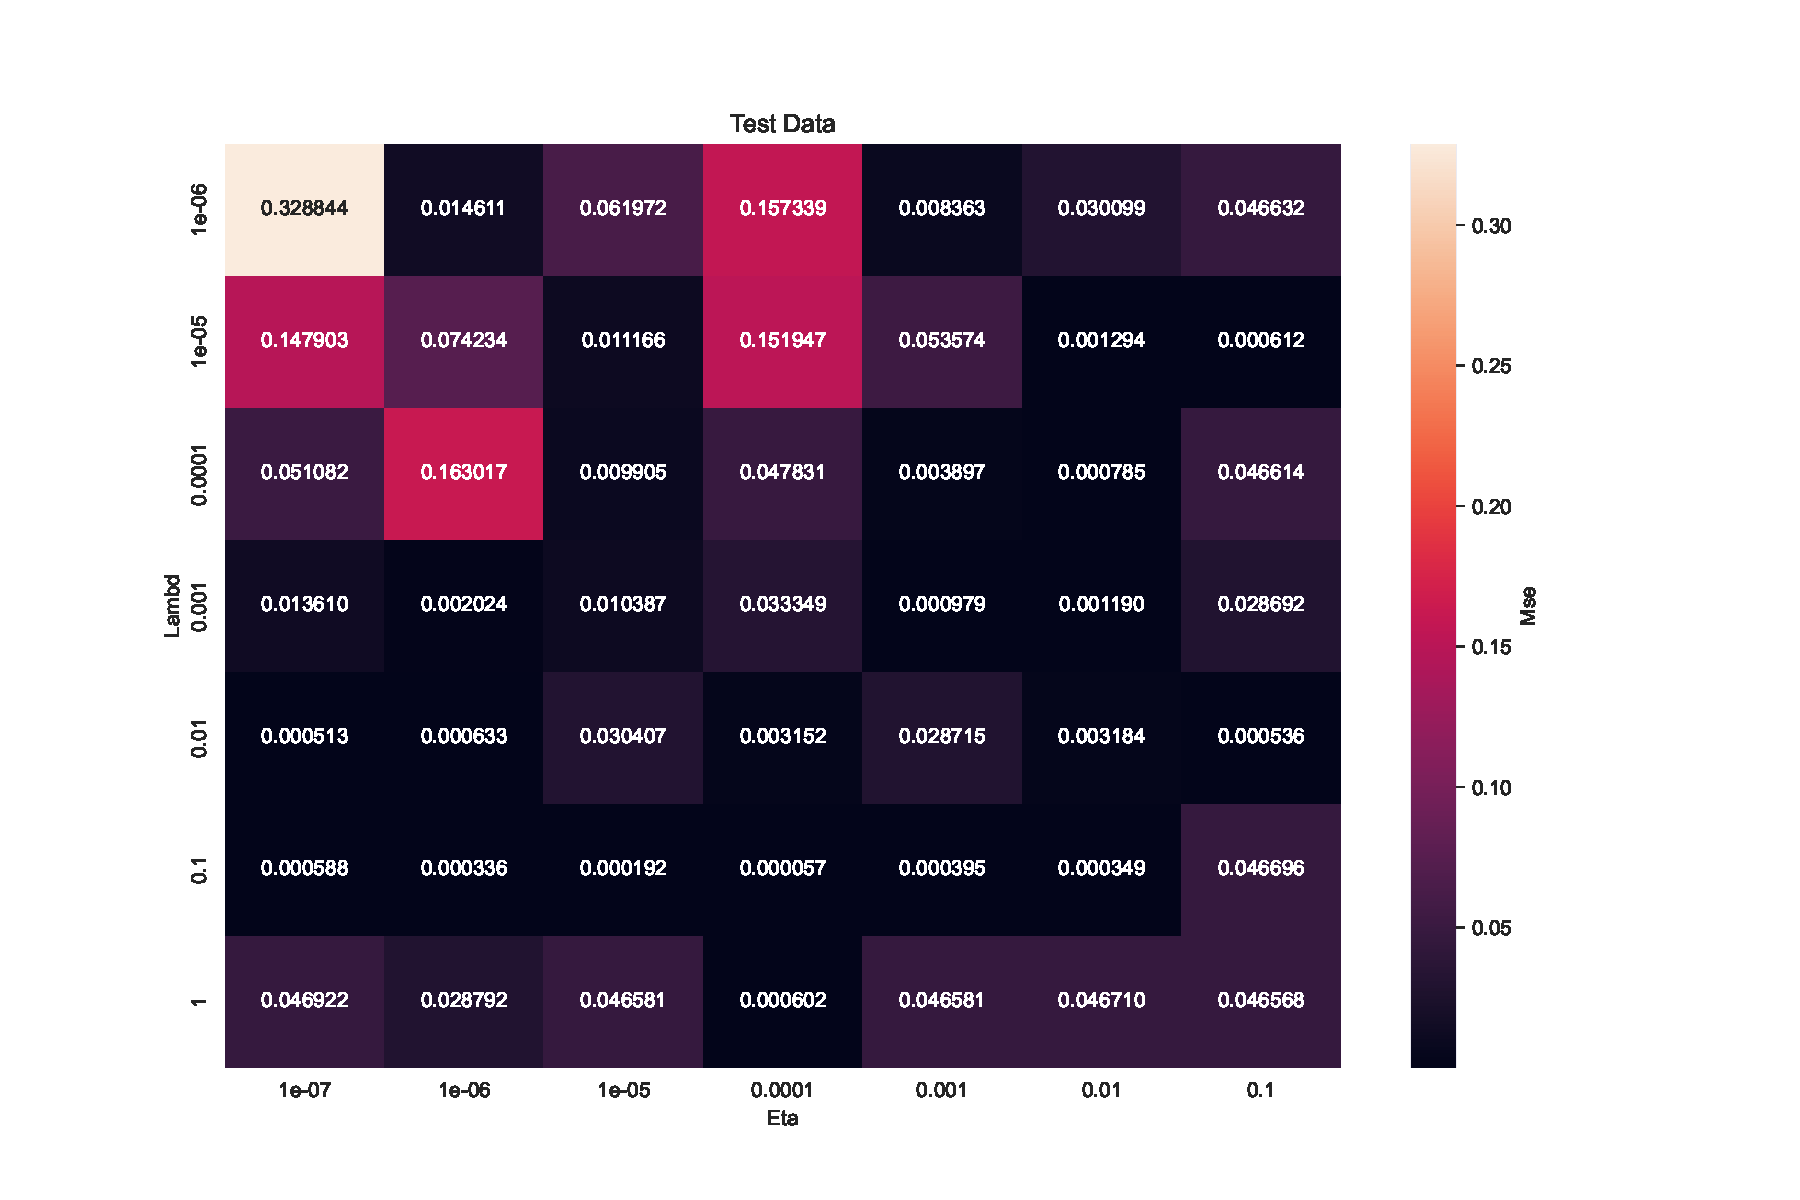
\includegraphics[width=1.2\linewidth]{Figures/PartB/test_relu_MSE(eta,lmb)}
  \caption{Test MSE}
  \label{fig:test_relu_MSE-eta-lmb-}
\end{subfigure}
\caption{Neural network with activation function relu MSE as a function of \(\eta \) and \(\lambda \) }
\label{fig:relu_MSE}
\end{figure}

\begin{figure}[htpb]
\begin{subfigure}{.5\textwidth}
  \centering
  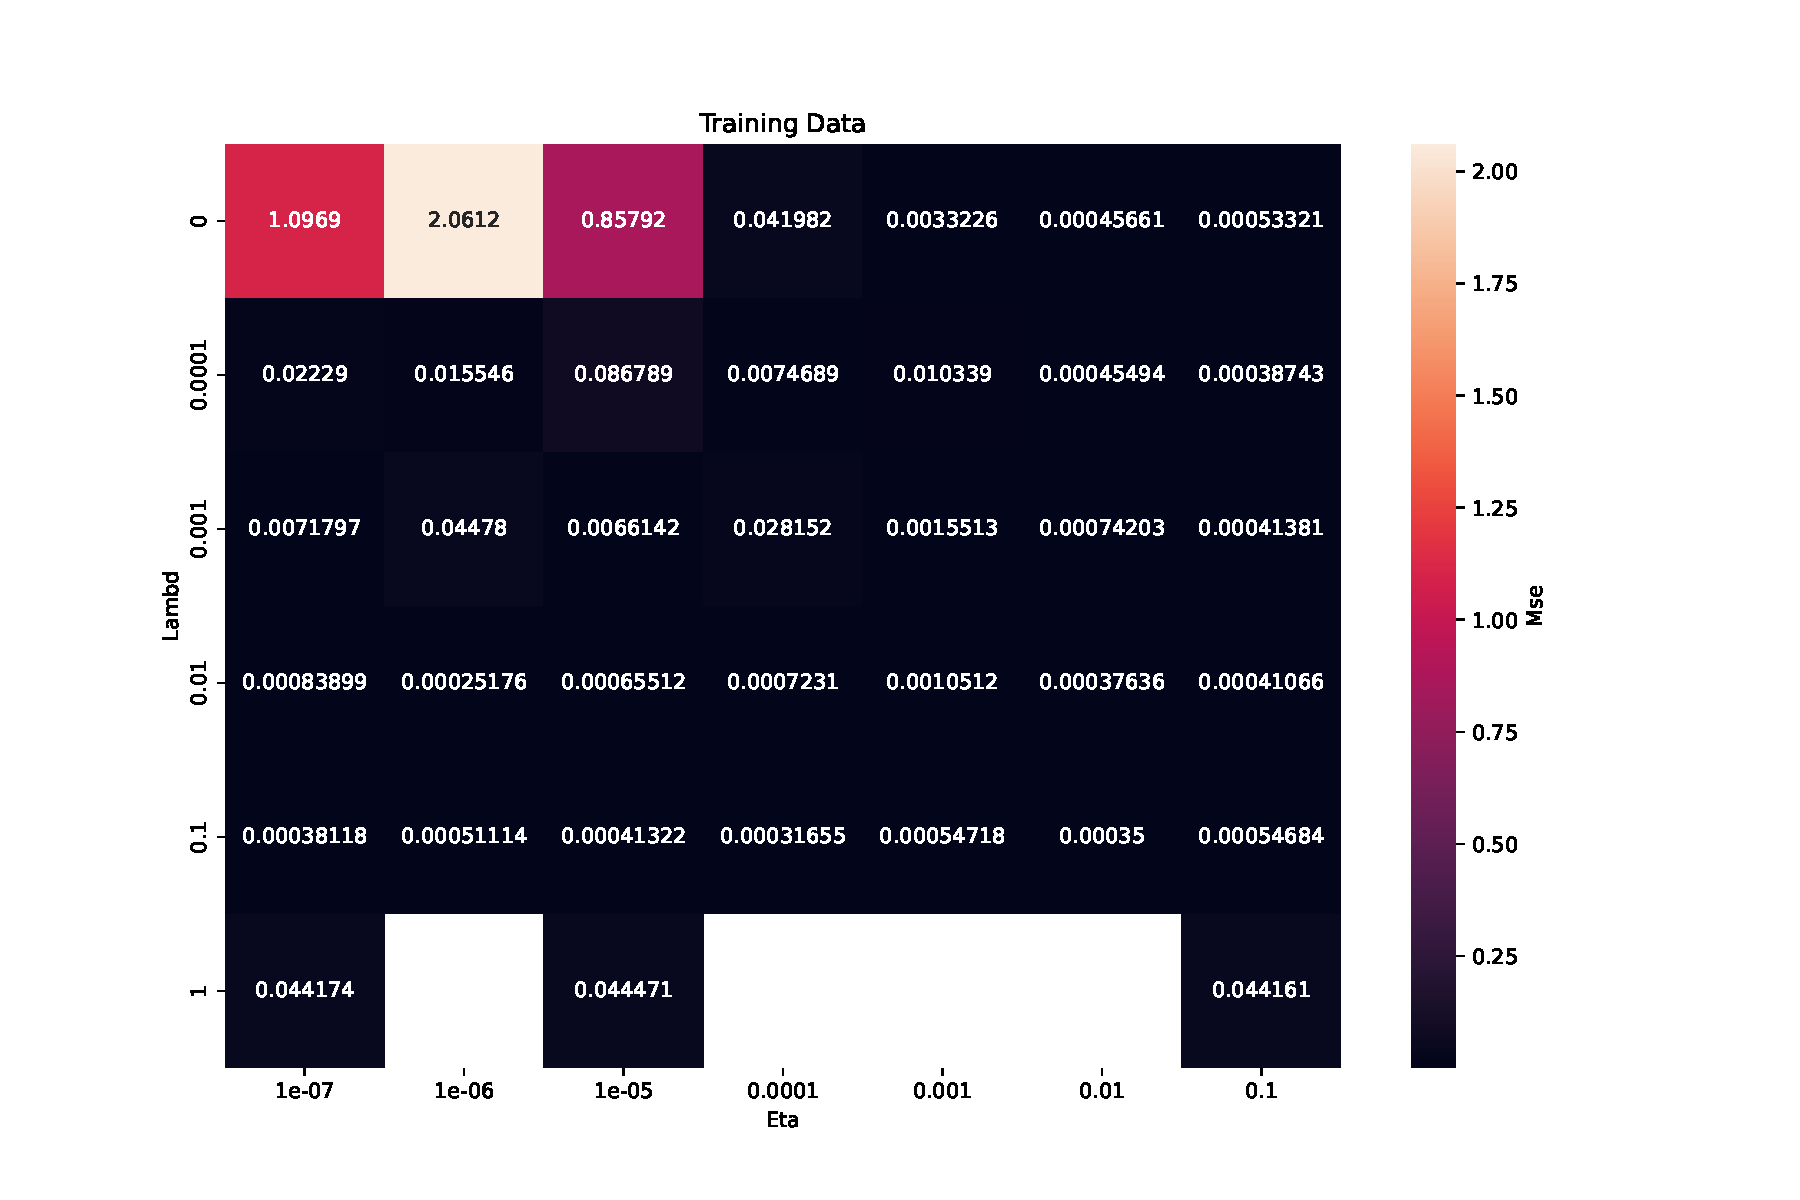
\includegraphics[width=1.2\linewidth]{Figures/PartB/train_leaky_relu_MSE(eta,lmb)}
  \caption{Train MSE}
  \label{fig:train_leaky_relu_MSE-eta-lmb-}
\end{subfigure}%
\begin{subfigure}{.5\textwidth}
  \centering
  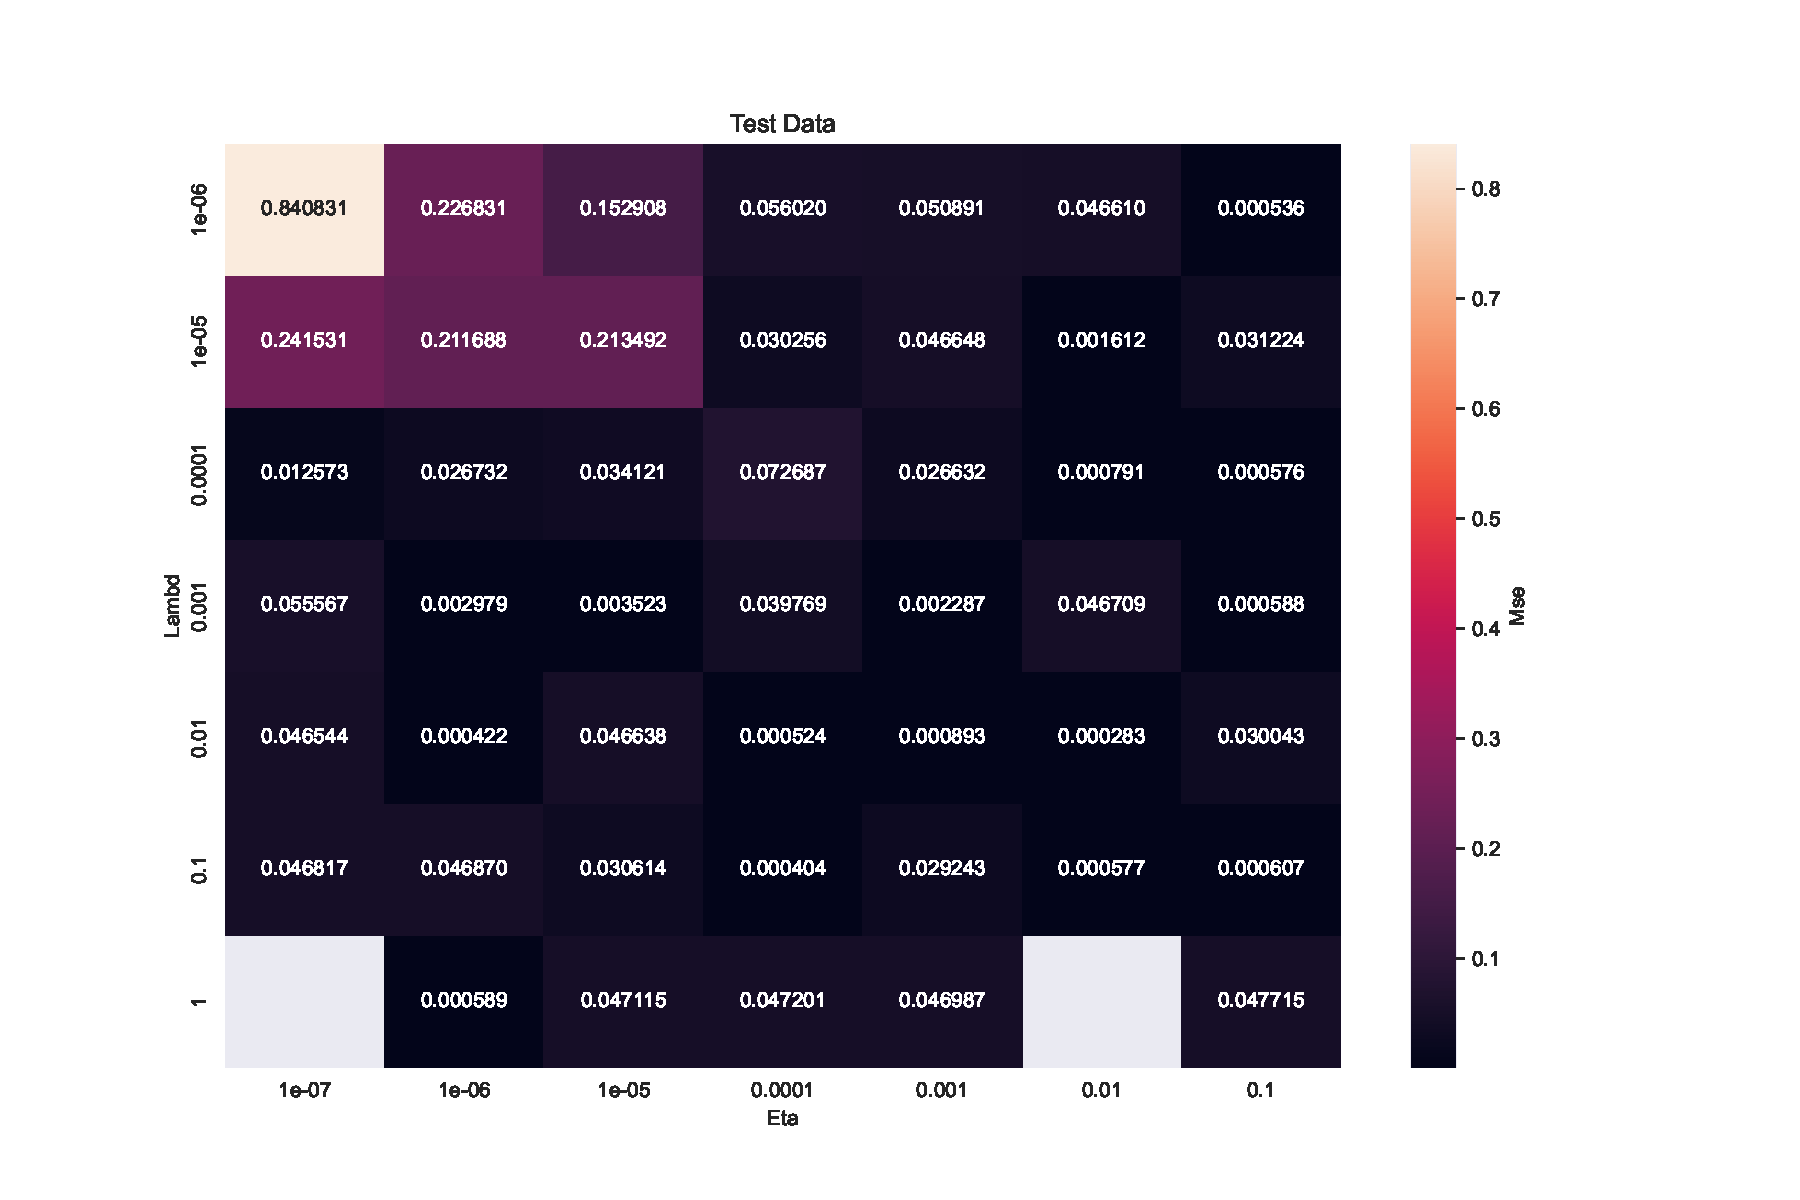
\includegraphics[width=1.2\linewidth]{Figures/PartB/test_leaky_relu_MSE(eta,lmb)}
  \caption{Test MSE}
  \label{fig:test_leaky_relu_MSE-eta-lmb-}
\end{subfigure}
\caption{Neural network with activation function leaky relu MSE as a function of \(\eta \) and \(\lambda \) }
\label{fig:leaky_relu_MSE}
\end{figure}






\subsection{Classification}


%  ____            _         _ 
% |  _ \ __ _ _ __| |_    __| |
% | |_) / _` | '__| __|  / _` |
% |  __/ (_| | |  | |_  | (_| |
% |_|   \__,_|_|   \__|  \__,_|
%                              

%%%%%%%%%%%%%%% Run 1 %%%%%%%%%%%%%%%
% Line plot with varying number of mini-batches

In figure \ref{fig:d_line_batch_size} the accuracy score is plotted for
different number of mini-batches. We observe that the convergence rate
increases with increasing number of mini-batches. This trend is expected. The
total amount of iterations/training is higher for a larger number for
mini batches. Another reason is that we are less likely to get stuck in global
minima, since the multiple different samples is used to calculate gradient of the
cost function. We also observe that the accuracy score tend to increase both
for the training and test data with increasing number of mini-batches.
We chose 20 number of mini-batches as our best value in the next. However, 15
number of mini-batches seems to give similar performance.    


\begin{figure}[H]
    \centering
    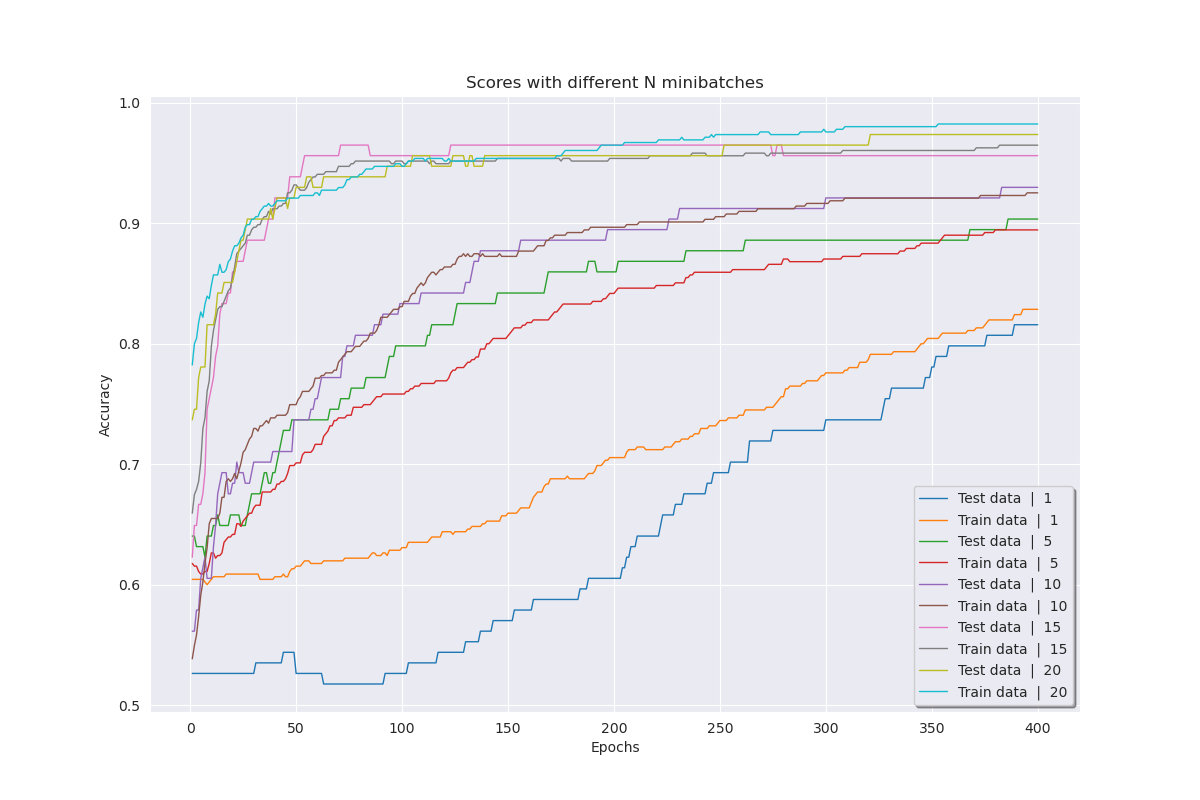
\includegraphics[width=0.8\textwidth]{Figures/PartD/d_line_batch_size.png}
    \caption{Accuracy score for train and test data plottet with respect to epochs for Run 1 (see table
    \ref{tab:runs_classification_cancer}). The number on the labels correspond
to number of mini-batches.}  
    \label{fig:d_line_batch_size} 
\end{figure}


%%%%%%%%%%%%%%% Run 2 %%%%%%%%%%%%%%%
% Lambda vs eta


In figure \ref{fig:d_heatmap_train_eta_vs_lambda} and
\ref{fig:d_heatmap_test_eta_vs_lambda} is accuracy score for run 2 plotted for
different values of regularization parameter and learning rate for the training
and test data respectively. For our test data the best Accuracy of 0.9825 was
gotten with $\lambda = 10^{-4}$, $\eta = 0.1$ and $\lambda = 0.01$, $\eta =
0.01$. Generally we observe that the accuracy tend to increase with increasing
learning rate. This make sense since the model is learning faster. High
learning rates often leads exploding loss scores. This is not observed in this
case. By choosing the largest learning rate, we can maximize the accuracy and
minimize CPU cycles. 

We observe an increasing trend in accuracy with respect to increasing $\lambda $
values (Lambda in figure). This is more significant for the smaller values
of learning rate. To further study this trend we plotted the accuracy score
for different $\lambda $ values with respect to epochs in figure
\ref{fig:_d_line_different_lambdas}. We clearly see in increased convergence
rate for higher values of lambda. Moreover, the accuracy both for the train and
test data is higher for larger values of $\lambda $. For further fine-tuning of
parameters we will set $\lambda = 0$, to better observe how the different
parameters affect the score with respect to epochs. 


% FIXME: fix figures, 

\begin{figure}[H]
    \centering
    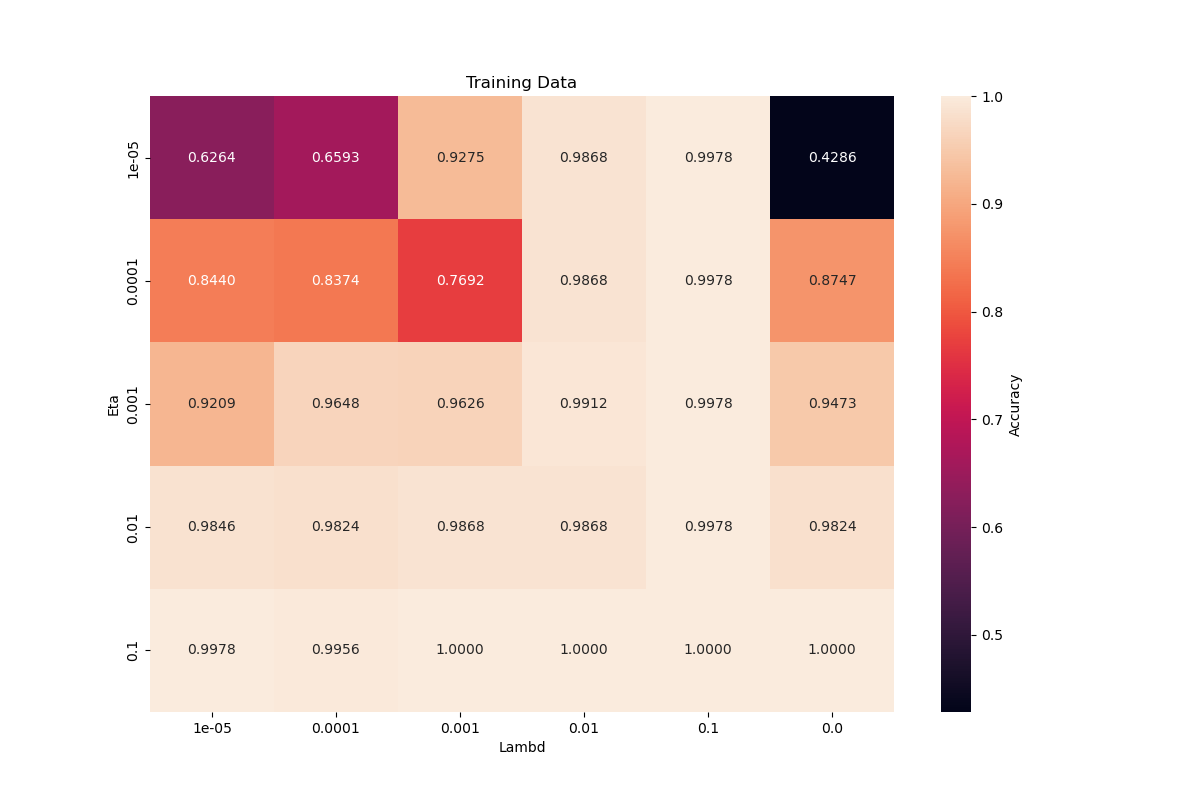
\includegraphics[width=\textwidth]{Figures/PartD/d_heatmap_train_eta_vs_lambda}
    \caption{Heatmap of accuracy score for training dta after 200 epochs with
    respect to different learning rates (Eta) and different L2-regularzation
    parameters (Lambd).   Spesific parameters used in run 2 is listed in table
\ref{tab:runs_classification_cancer}   }  
    \label{fig:d_heatmap_train_eta_vs_lambda}  
\end{figure}

\begin{figure}[H]
    \centering
    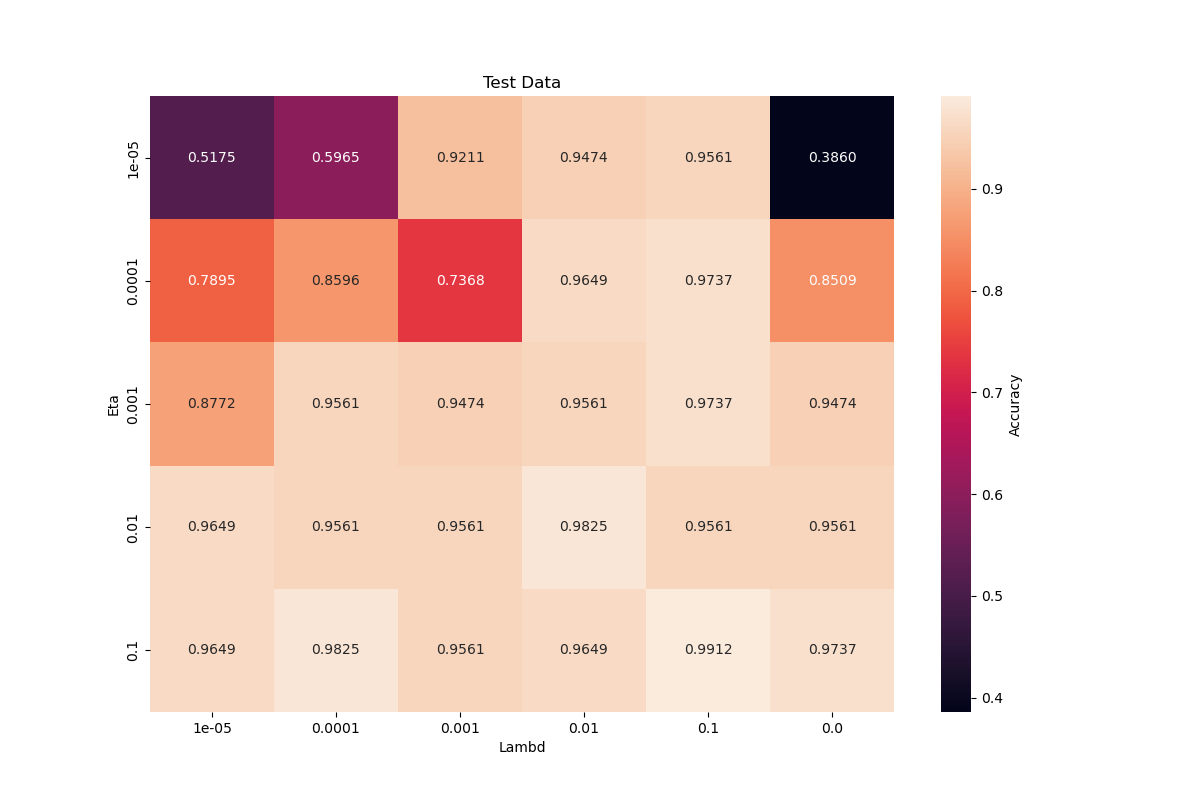
\includegraphics[width=\textwidth]{Figures/PartD/d_heatmap_test_eta_vs_lambda}
    \caption{Heatmap of accuracy score for test dta after 200 epochs with
    respect to different learning rates (Eta) and differn L2-regularization
    parameters (Lambd). Specific parameters used in run 2 is listed in table
    \ref{tab:runs_classification_cancer}       }  
    \label{fig:d_heatmap_test_eta_vs_lambda}  
\end{figure}


            
\begin{figure}[H]
    \centering
    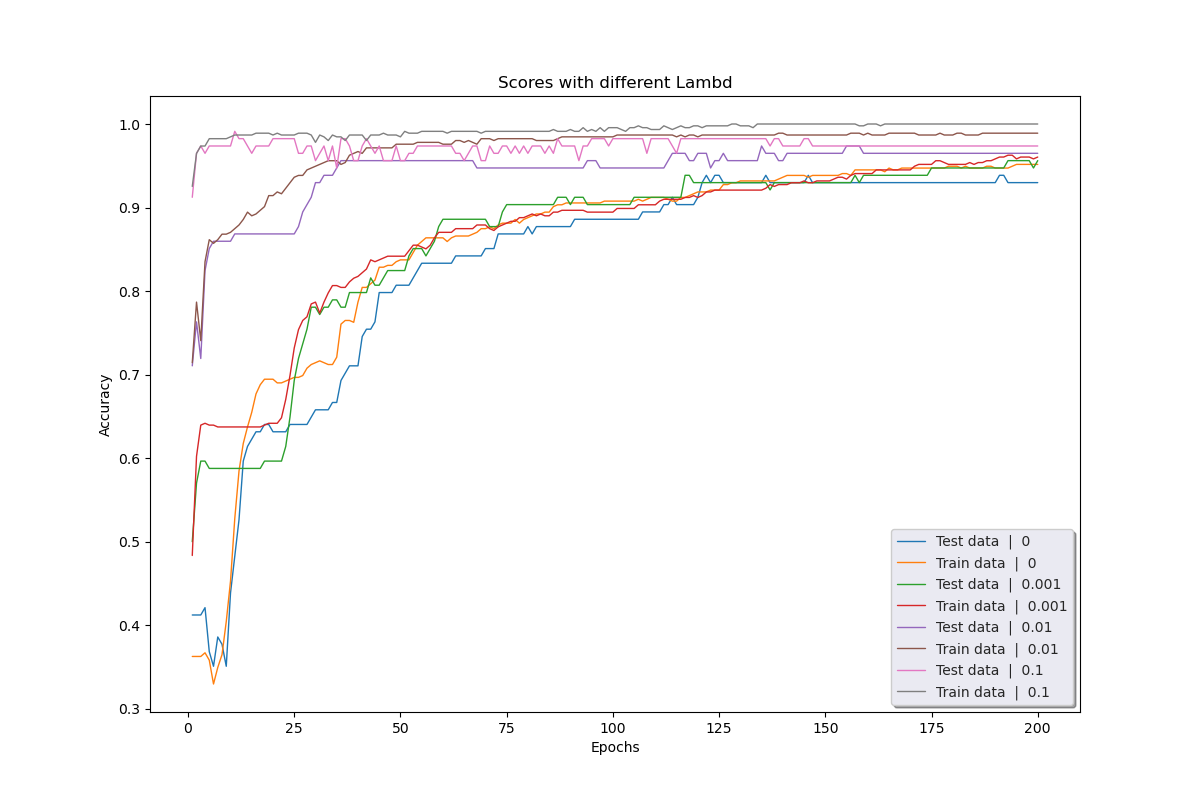
\includegraphics[width=0.8\textwidth]{Figures/PartD/_d_line_different_lambdas.png}
    \caption{Plot of accuracy score for training and test data with respect to
    epochs. Each line correspond to different values of $\lambda $ as indicated
by the number in the legend. A learning rate of 0.001 was used.}  
\label{fig:_d_line_different_lambdas} 
\end{figure}


%%%%%%%%%%%%%%% Run 3 %%%%%%%%%%%%%%%
% Depth vs width


In Run 3 different network architecture was tested with respect number of nodes
(width) and number of hidden layers (depth). The heat map's for the train and test
data is shown in figure \ref{fig:d_heatmap_train_depth_vs_width_lambd_0} and
\ref{fig:_d_heatmap_test_depth_vs_width_lambd_0}. For our test data the best
accuracy score was gotten with 2 hidden layers with 5 nodes in each, with an
accuracy of 0.9912. There is no clear trend with respect to architecture. We
will chose 2 hidden layers and 5 hidden nodes as our best parameters. However
the variations with respect to depth and width, may bet attributed to other random
phenomena such as mini-batch selection. There is no reason to chose a more
complex model since this will increase the computational cost of the network.      

% FIXME: not discussed training data


\begin{figure}[H]
    \centering
    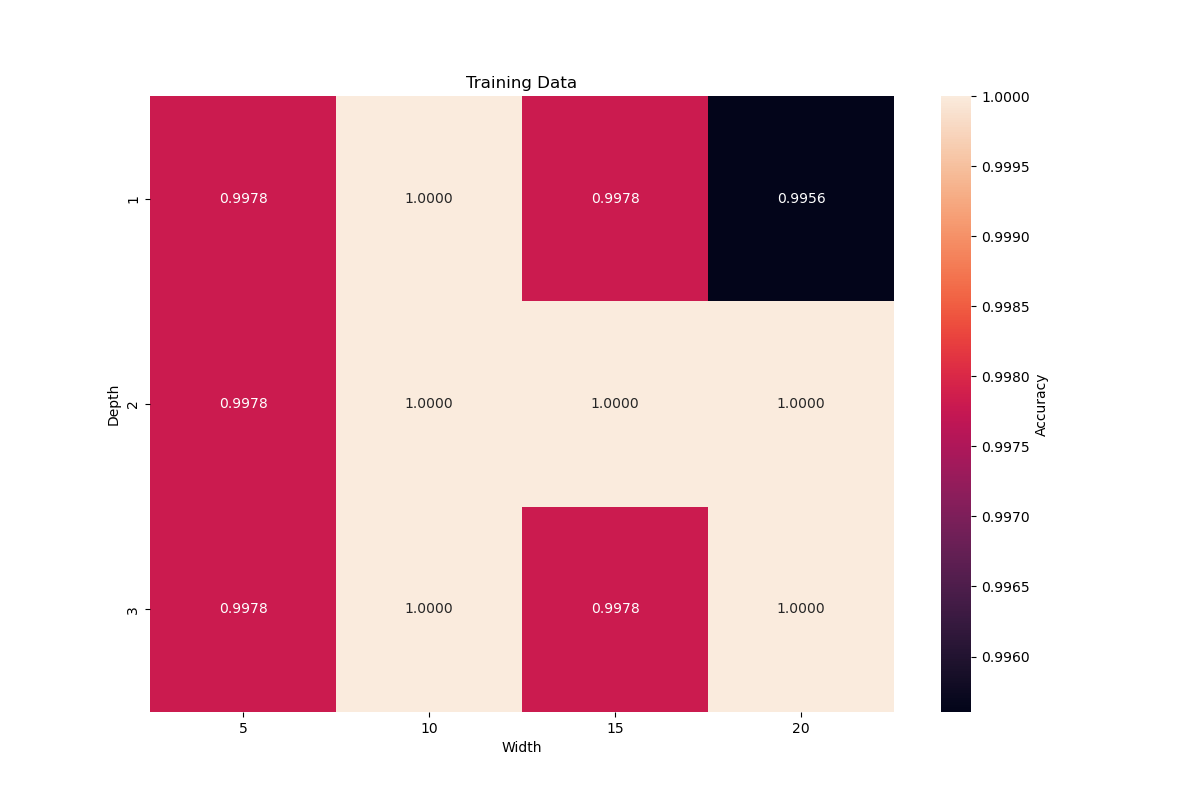
\includegraphics[width=0.8\textwidth]{Figures/PartD/d_heatmap_train_depth_vs_width_lambd_0.png}
    \caption{Accuracy score for train data with respect to different N number
        of hidden layers (depth) and number of hidden nodes in each hidden layer
    (width)  }  
    \label{fig:d_heatmap_train_depth_vs_width_lambd_0} 
\end{figure}


\begin{figure}[H]
    \centering
    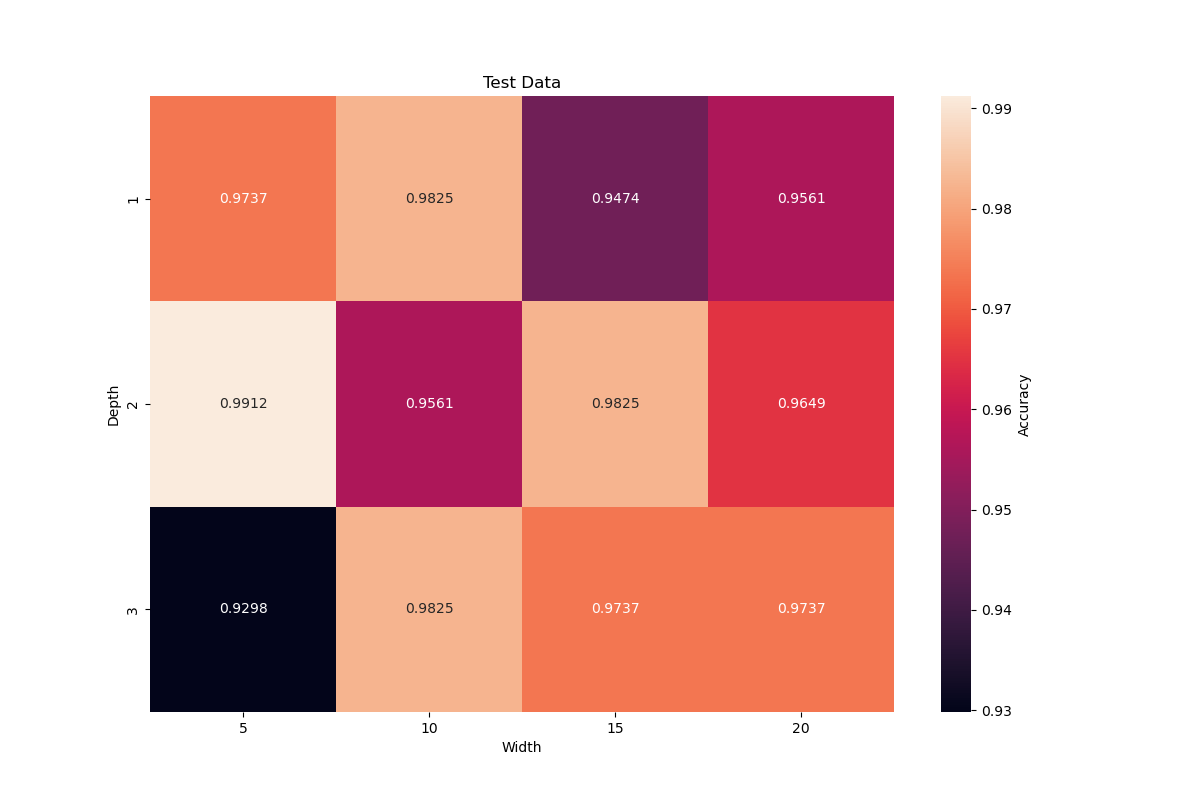
\includegraphics[width=0.8\textwidth]{Figures/PartD/_d_heatmap_test_depth_vs_width_lambd_0.png}
    \caption{Accuracy score for test data with respect to different N number
        of hidden layers (depth) and number of hidden nodes in each hidden layer
    (width)  }  
    \label{fig:_d_heatmap_test_depth_vs_width_lambd_0} 
\end{figure}

%%%%%%%%%%%%%%% Run 4 %%%%%%%%%%%%%%%
% Testing tuning method width and without momentum  

In Run 4 we tested different learning rate tuning methods. In figure
\ref{d_tuning_eta_0_001_with_gamma_0} the accuracy score is plotted
with respect to epochs for manual (none), adagrad, adman and the rms prop
tuning method. The learning rate parameter was set to 0.001. We observe that
RMS Prop and ADAM converges much faster than Adagrad and without any tuning.
The poor performance of Adgrad is probably due the low value initial value for
$\eta $. Both ADAM and RMS-prop performance well on both the training and test
data with a high accuracy and convergence after around 50 epochs. 

In figure \ref{fig:d_tuning_eta_0_001_with_gamma_0_9} the same lines are
plotted but with momentum, $\gamma = 0.9$. This causes a significant
improvement both the accuracy and convergence rate with Adagrad and plain SGD.   
Adagrad gives better prediction on the test data than both RMS prop and ADAM.
The added momentum to ADAM causes more fluctuations with respect to epochs than
without momentum.  

\begin{figure}[H]
    \centering
    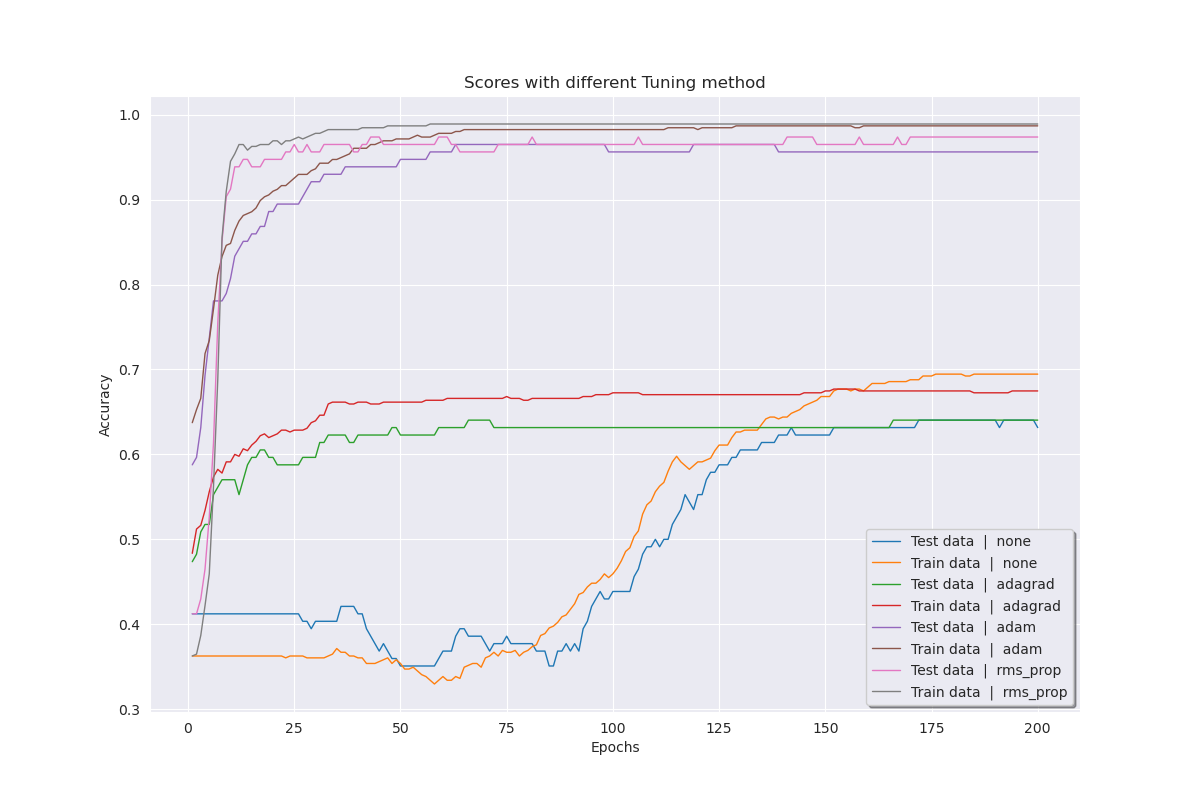
\includegraphics[width=0.8\textwidth]{Figures/PartD/d_tuning_eta_0_001_with_gamma_0.png}
    \caption{Accuracy score for test and data with different tuning methods
    plotted as function of epochs. Momentum ($\gamma $) is set to 0.}  
    \label{fig:d_tuning_eta_0_001_with_gamma_0_9} 
\end{figure}


\begin{figure}[H]
    \centering
    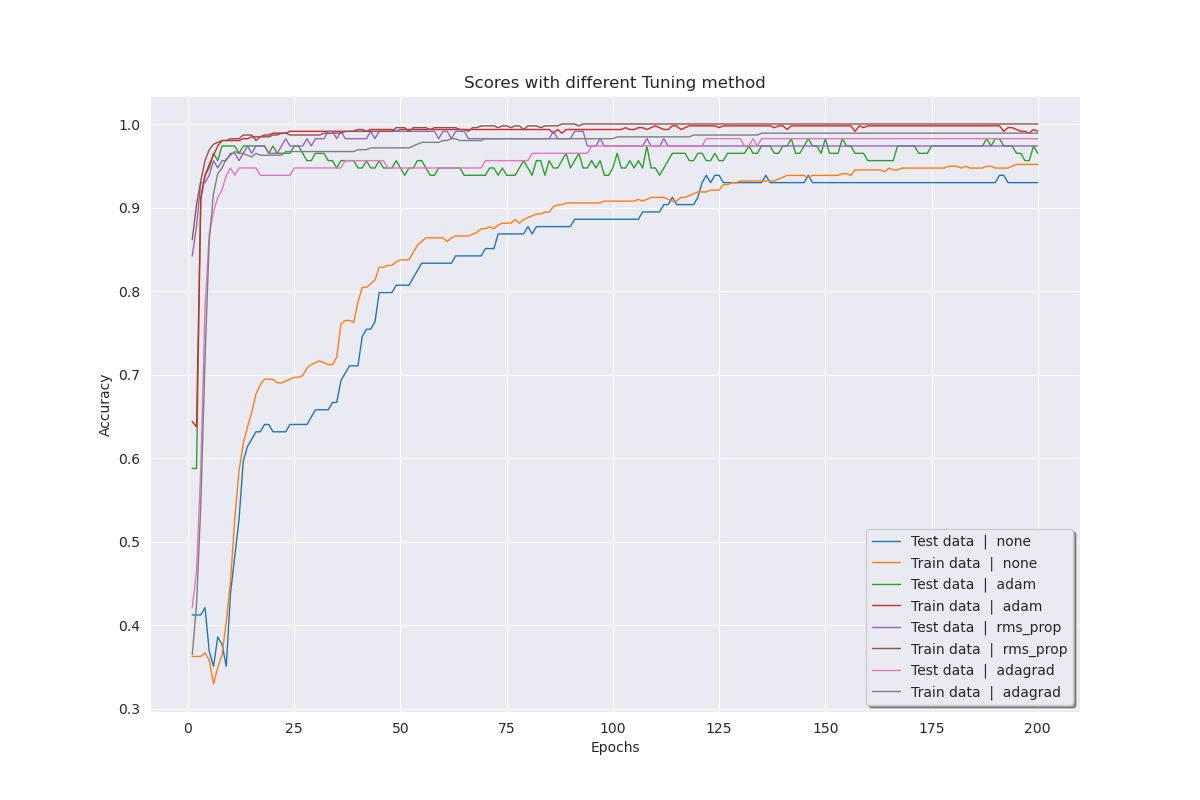
\includegraphics[width=0.8\textwidth]{Figures/PartD/d_tuning_eta_0_001_with_gamma_0_9.png}
    \caption{Accuracy score for test and data with different tuning methods
    plotted as function of epochs. Momentum ($\gamma $) is set to 0.9.}  
    \label{fig:d_tuning_eta_0_001_with_gamma_0_9} 

\end{figure}

%%%%%%%%%%%%%%% Run 5 %%%%%%%%%%%%%%%
% Activation function on hidden layers 

In run 5 we tested different activation functions on the hidden. From run 4 we
observed that both tuning method and added momentum improved the results
significantly. To understand better the different activation functions affect
the results we used a momentum parameter $\gamma = 0$ with constant learning
rate, $\eta = 0.001$. In figure \ref{fig:d_line_activation_hidden_gamma_0} the
accuracy is plotted for different activation functions in the hidden layers.
Both RELU and leaky RELU outperforms the sigmoid activation function. RELU and
Leaky RELU performs similar on the training data, but RELU gives the best
overall accuracy on the test data. 


\begin{figure}[H]
    \centering
    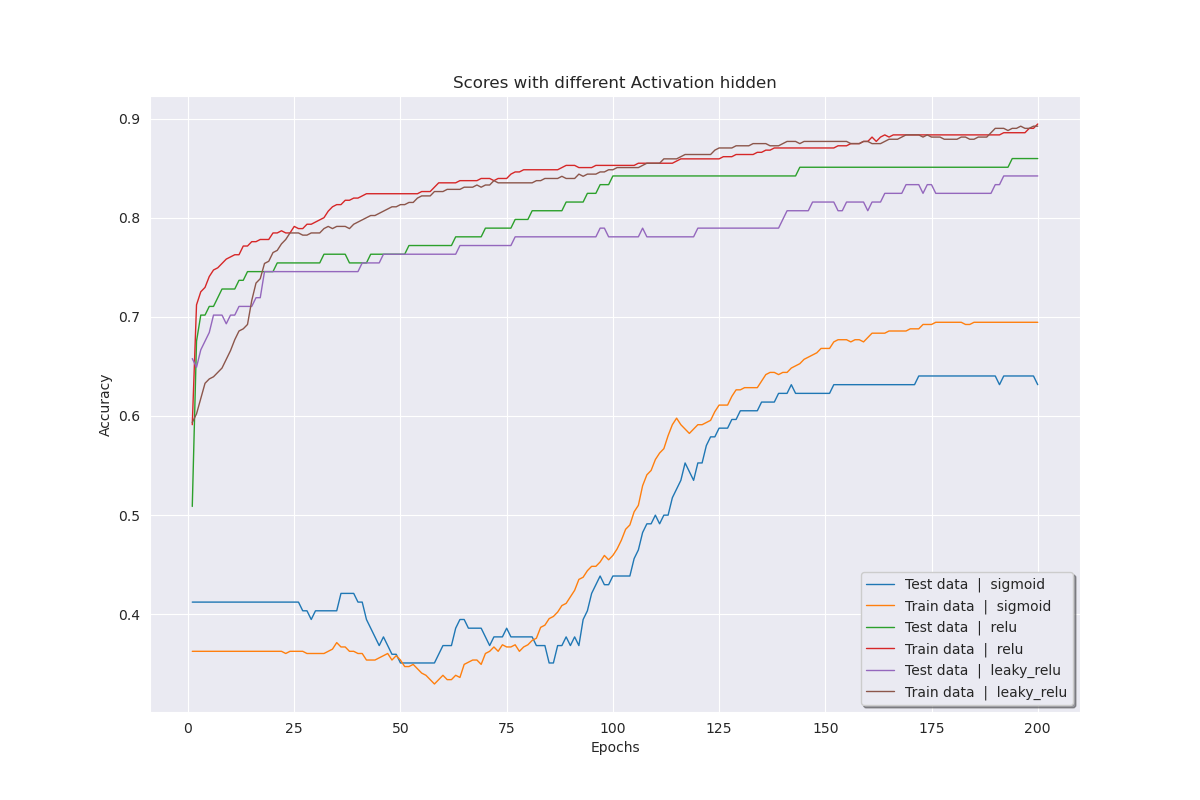
\includegraphics[width=0.8\textwidth]{Figures/PartD/d_line_activation_hidden_gamma_0.png}
    \caption{Accuracy score for train and test data with respect to epochs.
    Different activation functions on the hidden layers was used as indicated
in the label}  
\label{fig:d_line_activation_hidden_gamma_0} 
\end{figure}


%%%%%%%%%%%%%%% Run 6 %%%%%%%%%%%%%%%
% Combine best parameters

In run 6 our model reached an accuracy of 0.9825 after 165 epochs (see figure
\ref{fig:d_line_best}). The result was stable
with increasing number of iterations. We tried to select the optimal values for
hyper-parameters on the basis of the previous experimentation. However, we did
use the sigmoid function on the hidden layers and not REL or Leaky REL, as
they performed worse. The parameters used in run 6 is listed in table
\ref{tab:runs_classification_cancer2}. 

The overall best accuracy score on the test data seen in this experiment was observed in Run
3, where we experimented with different network architecture. Then we got a
score of 0.9912. We suspected that this was due to luck and random events in
our mini-batch selection method. 
% Compare with keras
Overall our model seemed to perform really well on a Classification problem
with the Wisconsin Breast Cancer data. We compared our results from run 6 with Kares
(python API for Tensor Flow), With the exact same parameters, except $\eta =
1$ and $\gamma = 0$. We then got a test accuracy prediction of 0.9825, that
matches our finding. 


% improvements
We originally tried to find the optimal parameters of the Network, by improving
a few parameters at the time. However, our best parameter choices created a
model with excellent predations after only a few epochs. Therefore, we decide
to remove some of the parameters to better be able to study how each individual
parameter affected the model. However, there is not certain that all the
parameters will play nicely together. Thus, a more methodical approach should
have been applied in order how different parameters affect each other.     

% To better control the randomness in our model we should have predefined a
% mini batch sequence, and also used the same initial weights when this was
% possible. Then we should have more easily seen if the variations in our
% predictions was due to random events or not. We did not study how the weights
% and bias initialization affected the results. 

From the literature we found
that models created with an artificial neural network and random forest
produces test accuracy's of 92.44 and 95.64 respectively \cite{Vig2014ComparativeAO}. Our model does a
better job on the test data. We don't expect our simple FINN code to be
superior to others. However, we do not suspect any error in implementation
since our benchmarking gave the same result.   

There is one serious drawback with our approach. We did not use any re-sampling
technique when we trained our model. Our high accuracy score is probably due to
our specific train-data subset selection. Bootstrap re-sampling would have been
a good choice to better control the randomness in our model. Then we would have
got better insight model variation due to parameter selection, and not random
events. However, this approach would have been too expensive for our
laptops. Therefore, a re-sampling technique such as k-fold cross validation
should have been applied.  


\begin{figure}[H]
    \centering
    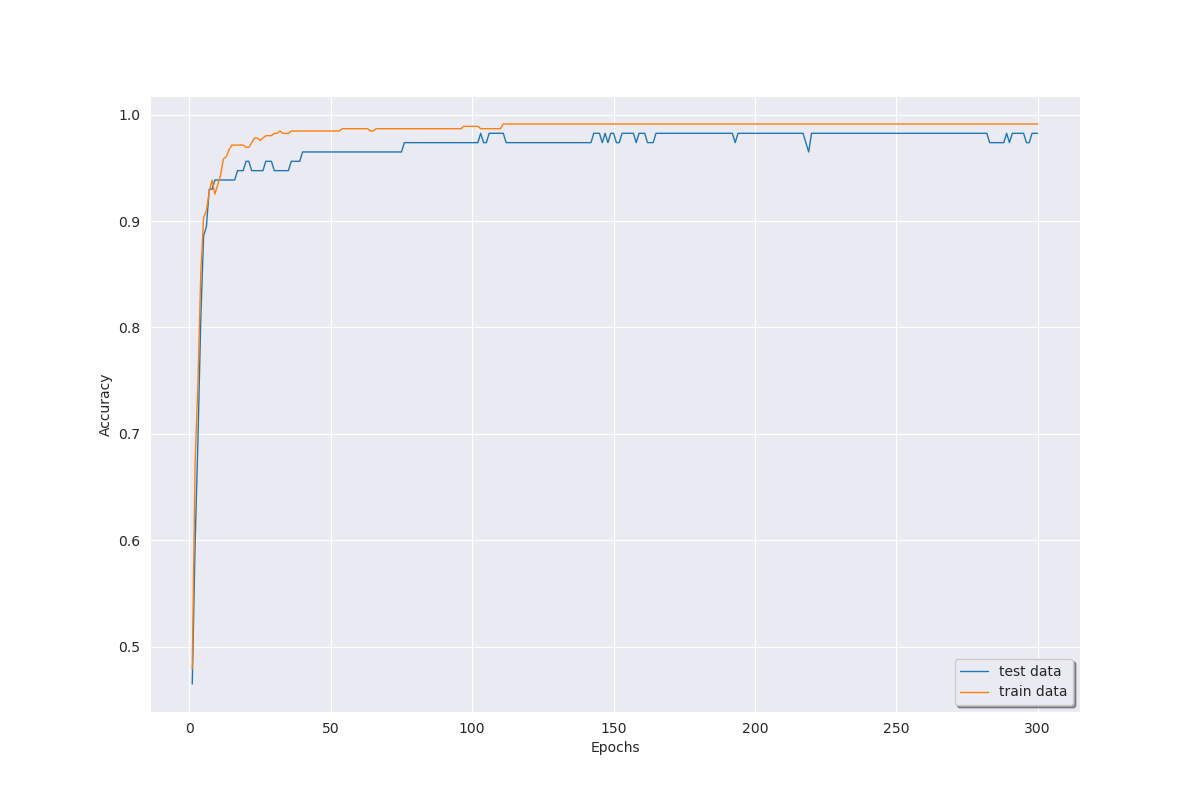
\includegraphics[width=0.8\textwidth]{Figures/PartD/d_line_best.png}
    \caption{Run 6: Plot of accuracy score for train and test data, where we
    tried to find the overall best hyper-parameter combination}  
    \label{fig:d_line_best} 
\end{figure}


After all these calculations there is only a few obvious choices for
hyper-parameters. A larger number of mini-batches did increase the accuracy,
convergence rate and reduces CPU cycles. We did not observe any over-fitting in 
our model, but a larger value for lambda did increase the convergence rate.
There was no clear trend in accuracy score with respect to network
architecture, but a depth of 2 and width of 5 gave the best prediction on the
test data. Tuning methods such as Adam and rms prop, significantly improved the
convergence rate. Adagrad and manual tuning was inferior to rms prop and adam,
but significantly improved when momentum was added. Adagrad then performed the
best on the test data. 


%  ____            _          
% |  _ \ __ _ _ __| |_    ___ 
% | |_) / _` | '__| __|  / _ \
% |  __/ (_| | |  | |_  |  __/
% |_|   \__,_|_|   \__|  \___|
                            

%%%%%%%%%%%%%%%%%%%%%%%%%%%%%%%%%%%%%%%%%%%%%
\subsection{Logistic regression}
% Study the results as functions of teh chosen learning rates 
% Add l2 regularization

In figure the accuracy score obtained with logistic regression is plotted for
different number of mini-batches. Again a small mini-batch size seems to be the
obvious choice as discussed for our neural network. In figure
\ref{fig:e_heatmap_train_lambd_vs_eta_gamma_0_9_epochs_200} and
\ref{fig:e_heatmap_test_lambd_vs_eta_gamma_0_9_epochs_200} the accuracy on the
Cancer Data is plotted with different learning rates and L2-regularization
parameters for the train and test data respectively. The best score for both
the training and test data was obtained with a learning rate $\eta = 0.001$
without any regularization. Our best prediction on the test data got an
accuracy of 0.9035. Our neural network code does contain 11 times as many
weights. Thus, we expect it to be able to produce more complex patterns. 
With did benchmark our result against scikit-learn's Logistic regression
method. We then got a test accuracy of  0.9649. We was not able to improve our
logistic regression algorithm to produce this result. We do not suspect that
our implementation is wrong. Scikit-learn's may contain further optimization.
Hence, the better accuracy score. However, our Neural Network did produce a
better accuracy score than Scikit-learns logistic regression method.

\begin{figure}[H]
    \centering
    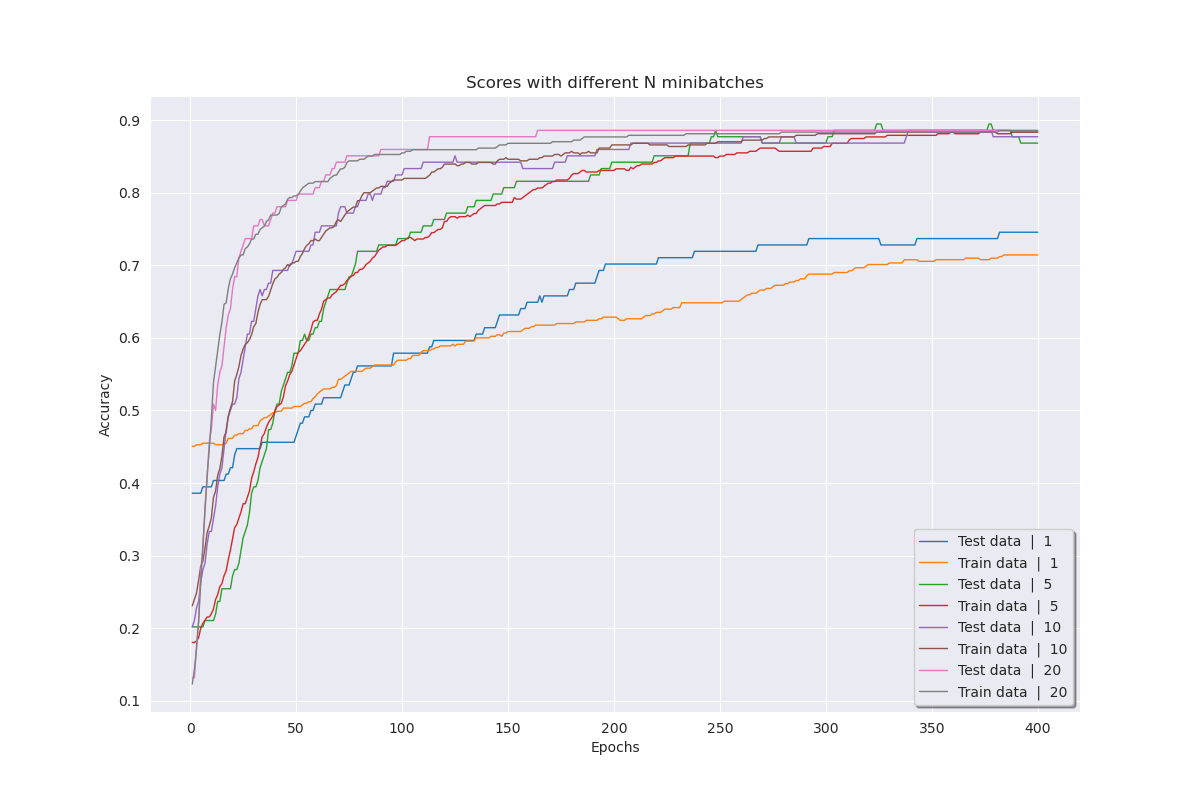
\includegraphics[width=0.8\textwidth]{Figures/PartE/e_line_n_minibatches_gamma_0_9.png}
    \caption{fig:Accuracy score obtained with logistic regression on the
        Wisconsin Breast Cacner data. Predication on training and test data is
    plotted for different number of mini-batches as indicated in the label.}  
    \label{fig:e_line_n_minibatches_gamma_0_9} 

\end{figure}

\begin{figure}[H]
    \centering
    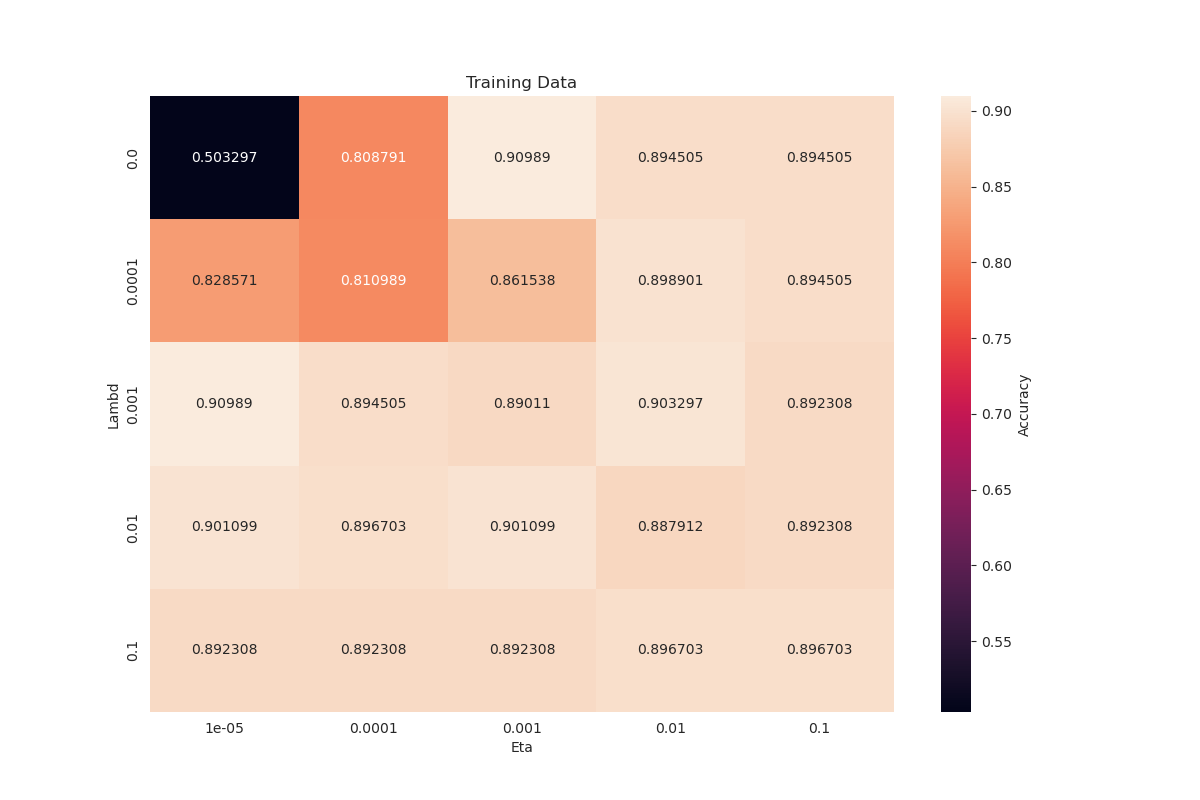
\includegraphics[width=0.8\textwidth]{Figures/PartE/e_heatmap_train_lambd_vs_eta_gamma_0_9_epochs_200.png}
    \caption{Accuracy score on Wisconsin Breast Cancer training data, with
    respect to different learning rates and L2 regularization parameters.}  
    \label{fig:e_heatmap_train_lambd_vs_eta_gamma_0_9_epochs_200} 
\end{figure}


\begin{figure}[H]
    \centering
    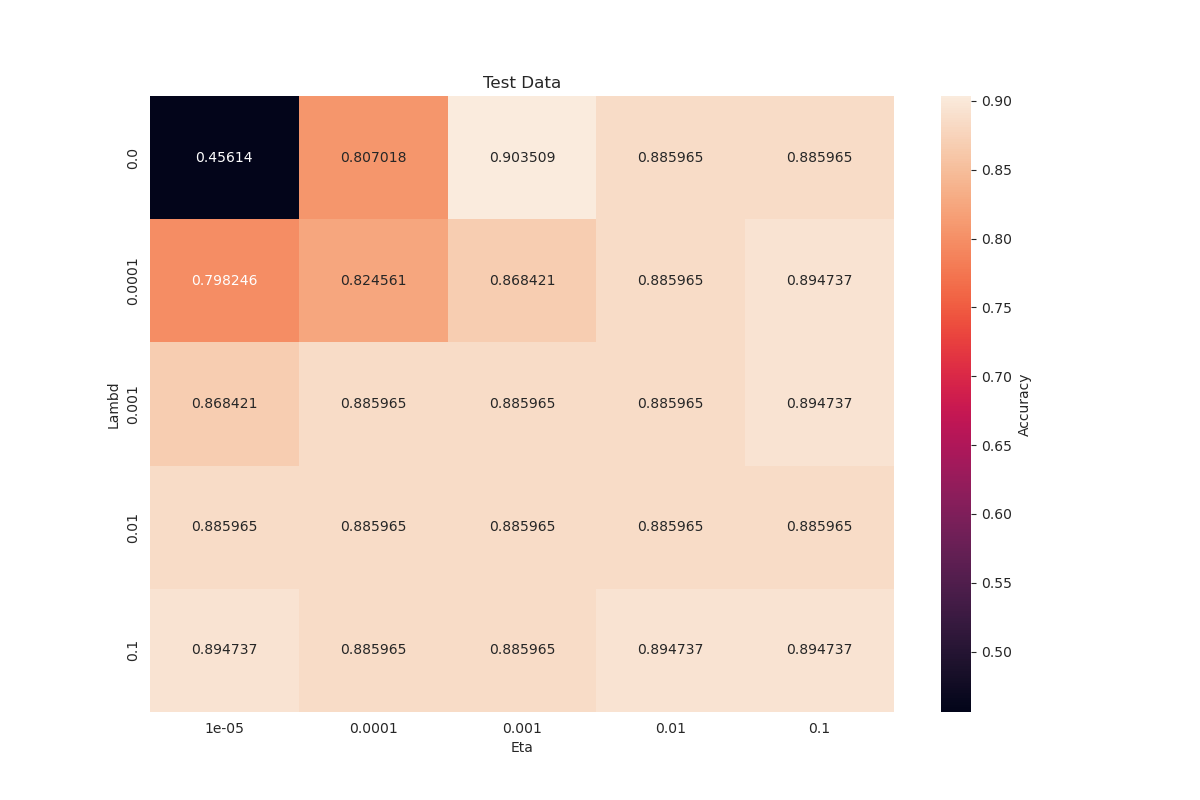
\includegraphics[width=0.8\textwidth]{Figures/PartE/e_heatmap_test_lambd_vs_eta_gamma_0_9_epochs_200.png}
    \caption{Accuracy score on Wisconsin Breast Cancer test data, with
    respect to different learning rates and L2 regularization parameters.}  
    \label{fig:e_heatmap_train_lambd_vs_eta_gamma_0_9_epochs_200} 
\end{figure}








\end{document}
